%!TEX root = SISC_elastic_3d.tex
\subsection{Gaussian source}\label{gaussian_source}
In this section, we perform a numerical simulation with a Gaussian source at the top surface and verify that  the curved mesh refinement interface does not generate any artifacts. 

We choose a flat top and bottom surface geometry 
\begin{equation*}
\theta_t\big(r^{(1)},r^{(2)}\big) = 1000,\quad \theta_b\big(r^{(1)},r^{(2)}\big) = 0,
\end{equation*}
respectively. The mesh refinement interface is parameterized by
\begin{equation}\label{interface_gausian}
\theta_i\big(r^{(1)},r^{(2)}\big) = 800+20\sin(4\pi r^{(1)})+20\cos(4\pi r^{(2)}),
\end{equation}
where $0\leq r^{(1)}, r^{(2)}, r^{(3)}\leq 1$. 
In addition, the mapping in the coarse domain $\Omega^c$ and fine domain $\Omega^f$ are given by 
\[ {\bf x} = {\bf X}^c({\bf r}) = \left(\begin{array}{c}
2000 r^{(1)}\\
2000 r^{(2)}\\
r^{(3)} \theta_i\big(r^{(1)}, r^{(2)}\big) + (1-r^{(3)}) \theta_b\big(r^{(1)},r^{(2)}\big) \end{array}\right) \]
and 
\[ {\bf x} = {\bf X}^f({\bf r}) = \left(\begin{array}{c}
2000 r^{(1)}\\
2000 r^{(2)}\\
r^{(3)}\theta_t\big(r^{(1)},r^{(2)}\big) + (1-r^{(3)})\theta_i\big(r^{(1)},r^{(2)}\big)\end{array}\right), \]
respectively. 
%For the coarse domain $\Omega^c$, the mapping is given by
%\[ {\bf x} = {\bf X}^c({\bf r}) = \left(\begin{array}{c}
%2000 r^{(1)}\\
%2000 r^{(2)}\\
%r^{(3)} \theta_i\big(r^{(1)}, r^{(2)}\big) + (1-r^{(3)}) \theta_b\big(r^{(1)},r^{(2)}\big) \end{array}\right). \]
%Here, $0\leq r^{(1)}, r^{(2)}, r^{(3)}\leq 1$, $\theta_i$ represents the interface surface geometry,
%\begin{equation}\label{interface_gausian}
%\theta_i\big(r^{(1)},r^{(2)}\big) = 800+20\sin(4\pi r^{(1)})+20\cos(4\pi r^{(2)}),
%\end{equation}
%and $\theta_b$ is the bottom surface geometry,
%\begin{equation*}
%\theta_b\big(r^{(1)},r^{(2)}\big) = 0.
%\end{equation*}
%As for the fine domain $\Omega^f$, the mapping is chosen to be
%\[ {\bf x} = {\bf X}^f({\bf r}) = \left(\begin{array}{c}
%2000 r^{(1)}\\
%2000 r^{(2)}\\
%r^{(3)}\theta_t\big(r^{(1)},r^{(2)}\big) + (1-r^{(3)})\theta_i\big(r^{(1)},r^{(2)}\big)\end{array}\right), \]
%where $0\leq r^{(1)}, r^{(2)}, r^{(3)}\leq 1$ and $\theta_t$ is the top surface geometry with
%\begin{equation*}
%\theta_t\big(r^{(1)},r^{(2)}\big) = 1000,
%\end{equation*}
%$\theta_i$ is the interface geometry which is given in (\ref{interface_gausian}). 
In the entire domain, we use the homogeneous material properties
%\begin{equation*}
%\rho(x^{(1)},x^{(2)},x^{(3)}) = 1.5\times 10^3,
%\end{equation*}
%and 
\begin{equation*}
\rho(x^{(1)},x^{(2)},x^{(3)}) = 1.5\times 10^3,\ \  \mu(x^{(1)},x^{(2)},x^{(3)}) = 1.5\times 10^9,\ \ 
\lambda(x^{(1)},x^{(2)},x^{(3)})  = 3\times 10^9.
\end{equation*}

At the top surface, the Gaussian source 
${\bf g} = (g_1,g_2,g_3)^T$ is imposed as the Dirichlet data with $g_1 = g_2 = 0$ and 
\[g_3 = 10^9 \text{exp}\left(-\left(\frac{t-4/44.2}{1/44.2}\right)^2\right)\text{exp}\left(-\left(\frac{x^{(1)}-1000}{12.5}\right)^2-\left(\frac{x^{(2)}-1000}{12.5}\right)^2\right).\]  
Homogeneous Dirichlet boundary conditions are imposed at other boundaries. Both the initial conditions and the external forcing are set to zero everywhere. % and the initial conditions are also set to be zero everywhere, ${\bf F}(\cdot,0) = {\bf C}(\cdot,0) = {\bf u}(\cdot,0) = {\bf 0}, {\bf u}(\cdot,t) = (u_1(\cdot,t), u_2(\cdot,t), u_3(\cdot,t))^T$.
For these material properties, the shear wave velocity is $c_s = \sqrt{\mu/\rho}=1000$. With the dominant wave frequency $f_0=44.2\sqrt{2}/(2\pi)\approx 10$, the wavelength $c_s/f_0$ is approximately 100.

In the numerical schemes, we consider three different meshes: Mesh 1 is the Cartesian mesh without any interface and $n_1 = n_2 = 201, n_3 = 101$ with $n_i$ denotes the number of grid points in the direction $x^{(i)}$. This corresponds to 10 grid points per wavelength and is considered as the  reference solution. Mesh 2 is the curvilinear mesh with a curved mesh refinement interface defined in \eqref{interface_gausian} and $n_1^{2h} = n_2^{2h} = 101, n_3^{2h} = 41$, $n_1^h = n_2^h = 201, n_3^h = 21$. The mesh size in $\Omega^f$ is approximately the same as the mesh size in the Cartesian mesh. As a result, the waves are resolved with 5 grid points per wavelength in $\Omega^c$. Mesh 3 is obtained by refining Mesh 2 in all three spatial directions. %The final simulation time is $T = 0.4$. %is a curvilinear mesh with the same curved mesh refinement interface and $n_1^{2h} = n_2^{2h} = 201, n_3^{2h} = 81$, $n_1^h = n_2^h = 401, n_3^h = 41$. We notice that the third mesh is a finer version of the second mesh. The final simulation time is $T = 0.4$.

\begin{figure}[htbp]
	\centering
	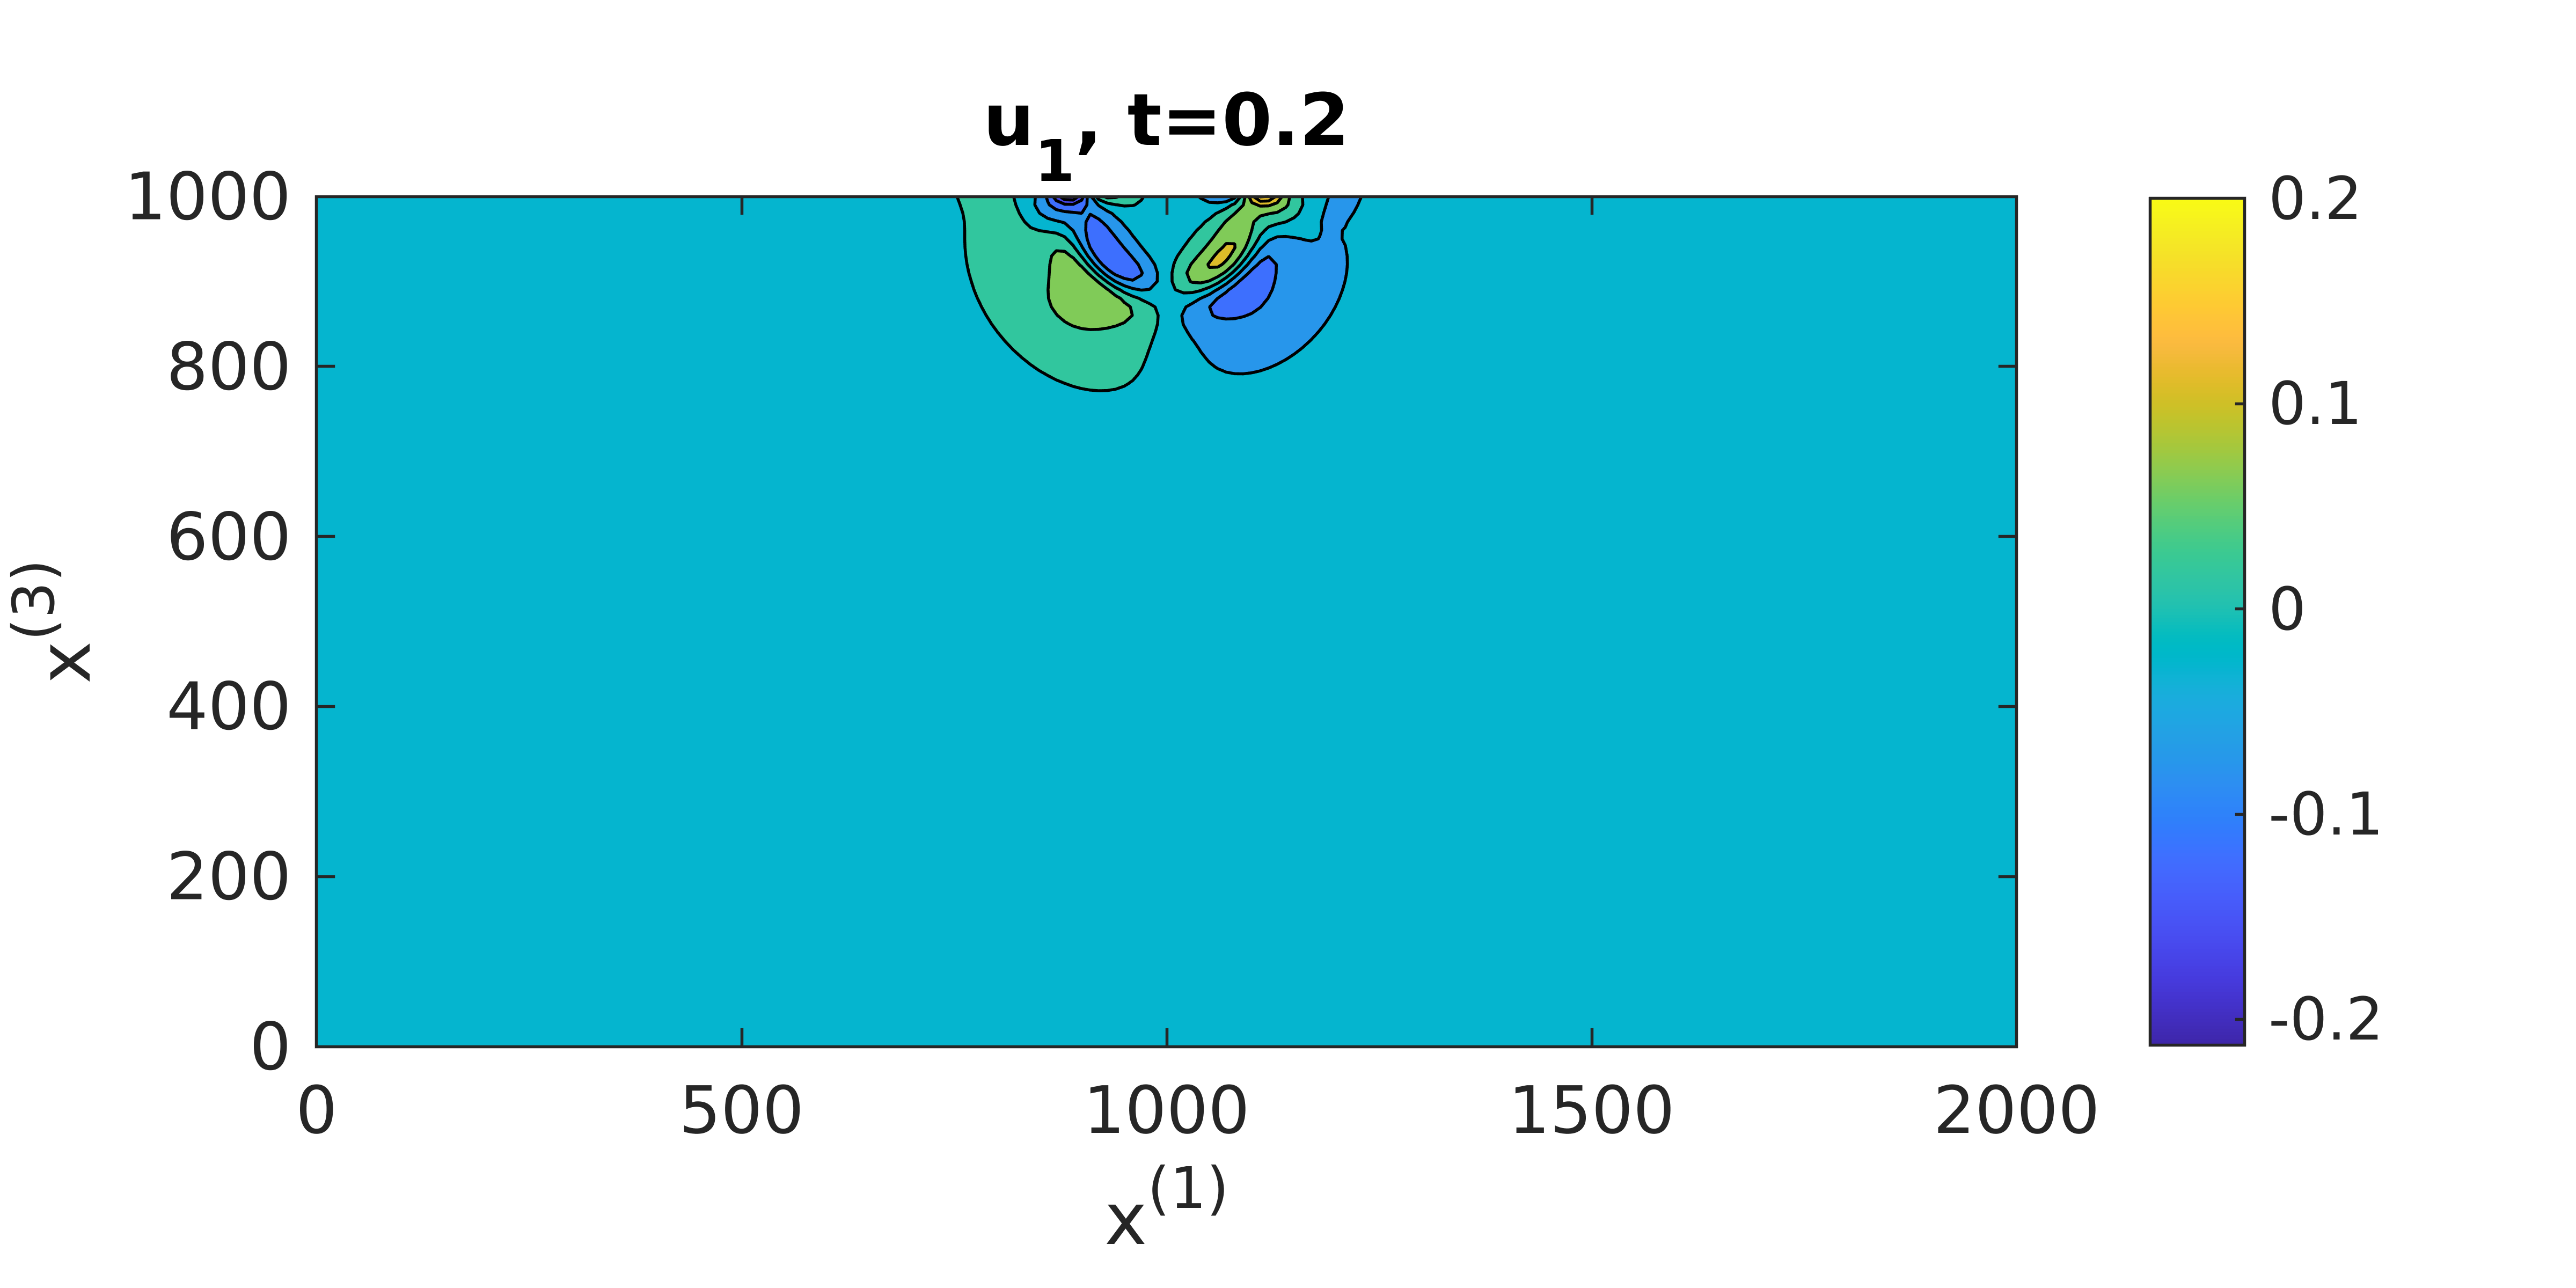
\includegraphics[width=0.49\textwidth,trim={0.05cm 0.1cm 0.55cm 0.45cm}, clip]{u1_t02_cartesian.png}
	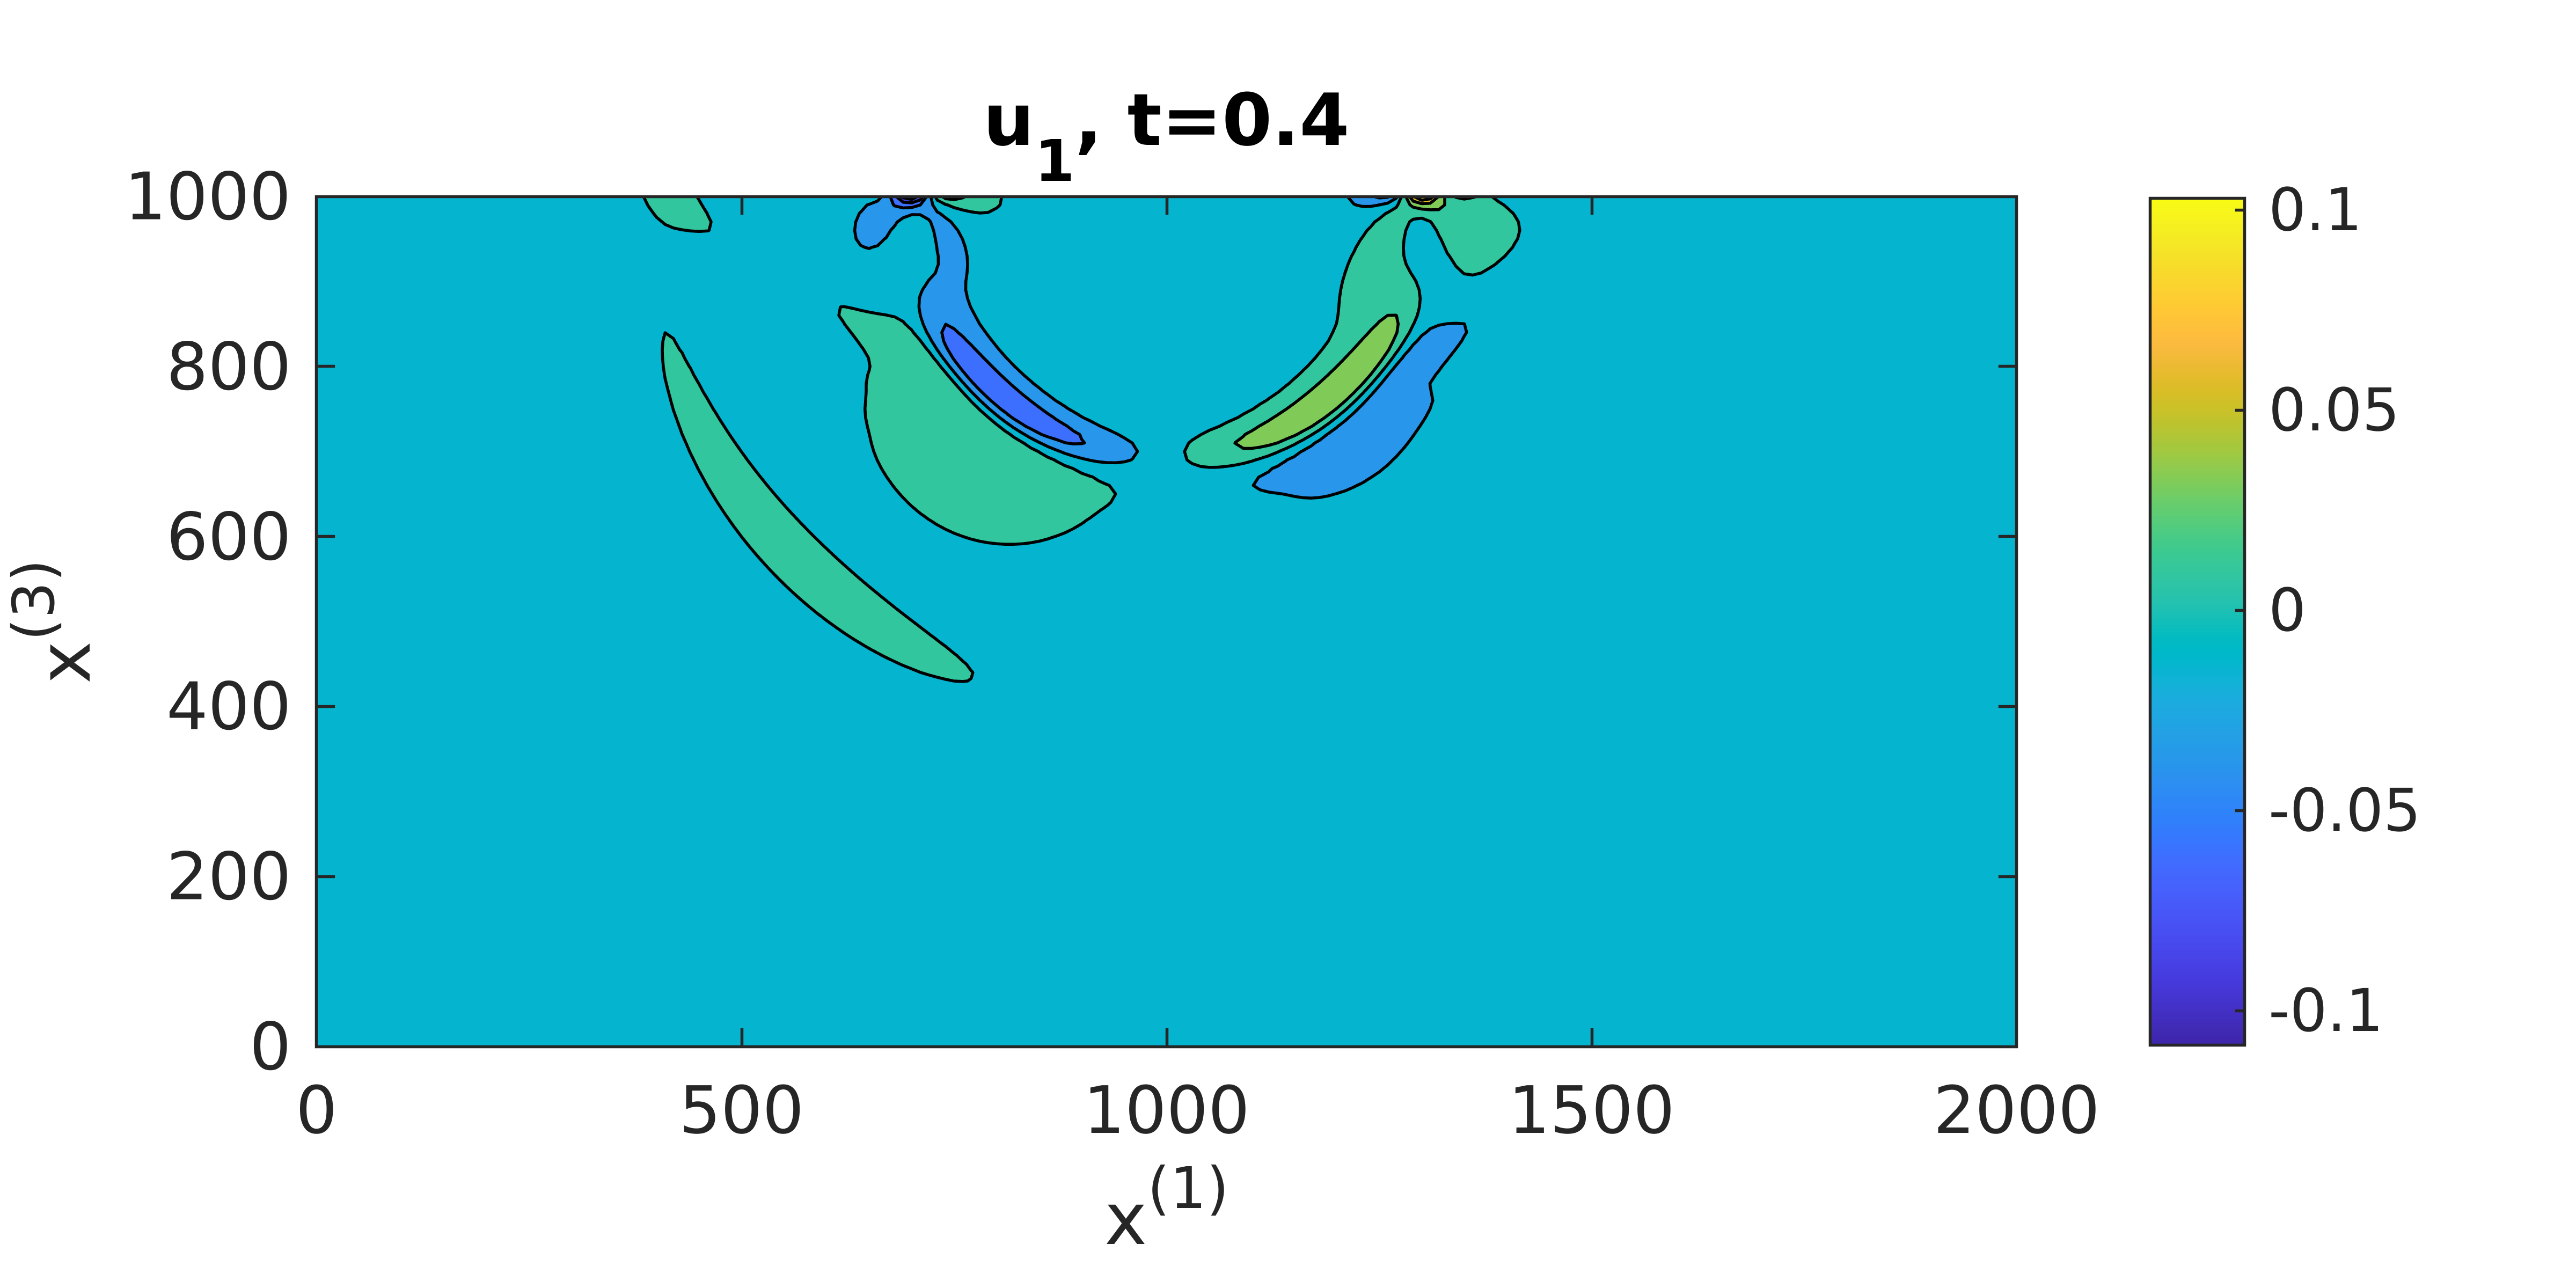
\includegraphics[width=0.49\textwidth,trim={0.05cm 0.1cm 0.55cm 0.45cm}, clip]{u1_t04_cartesian.png}\\
	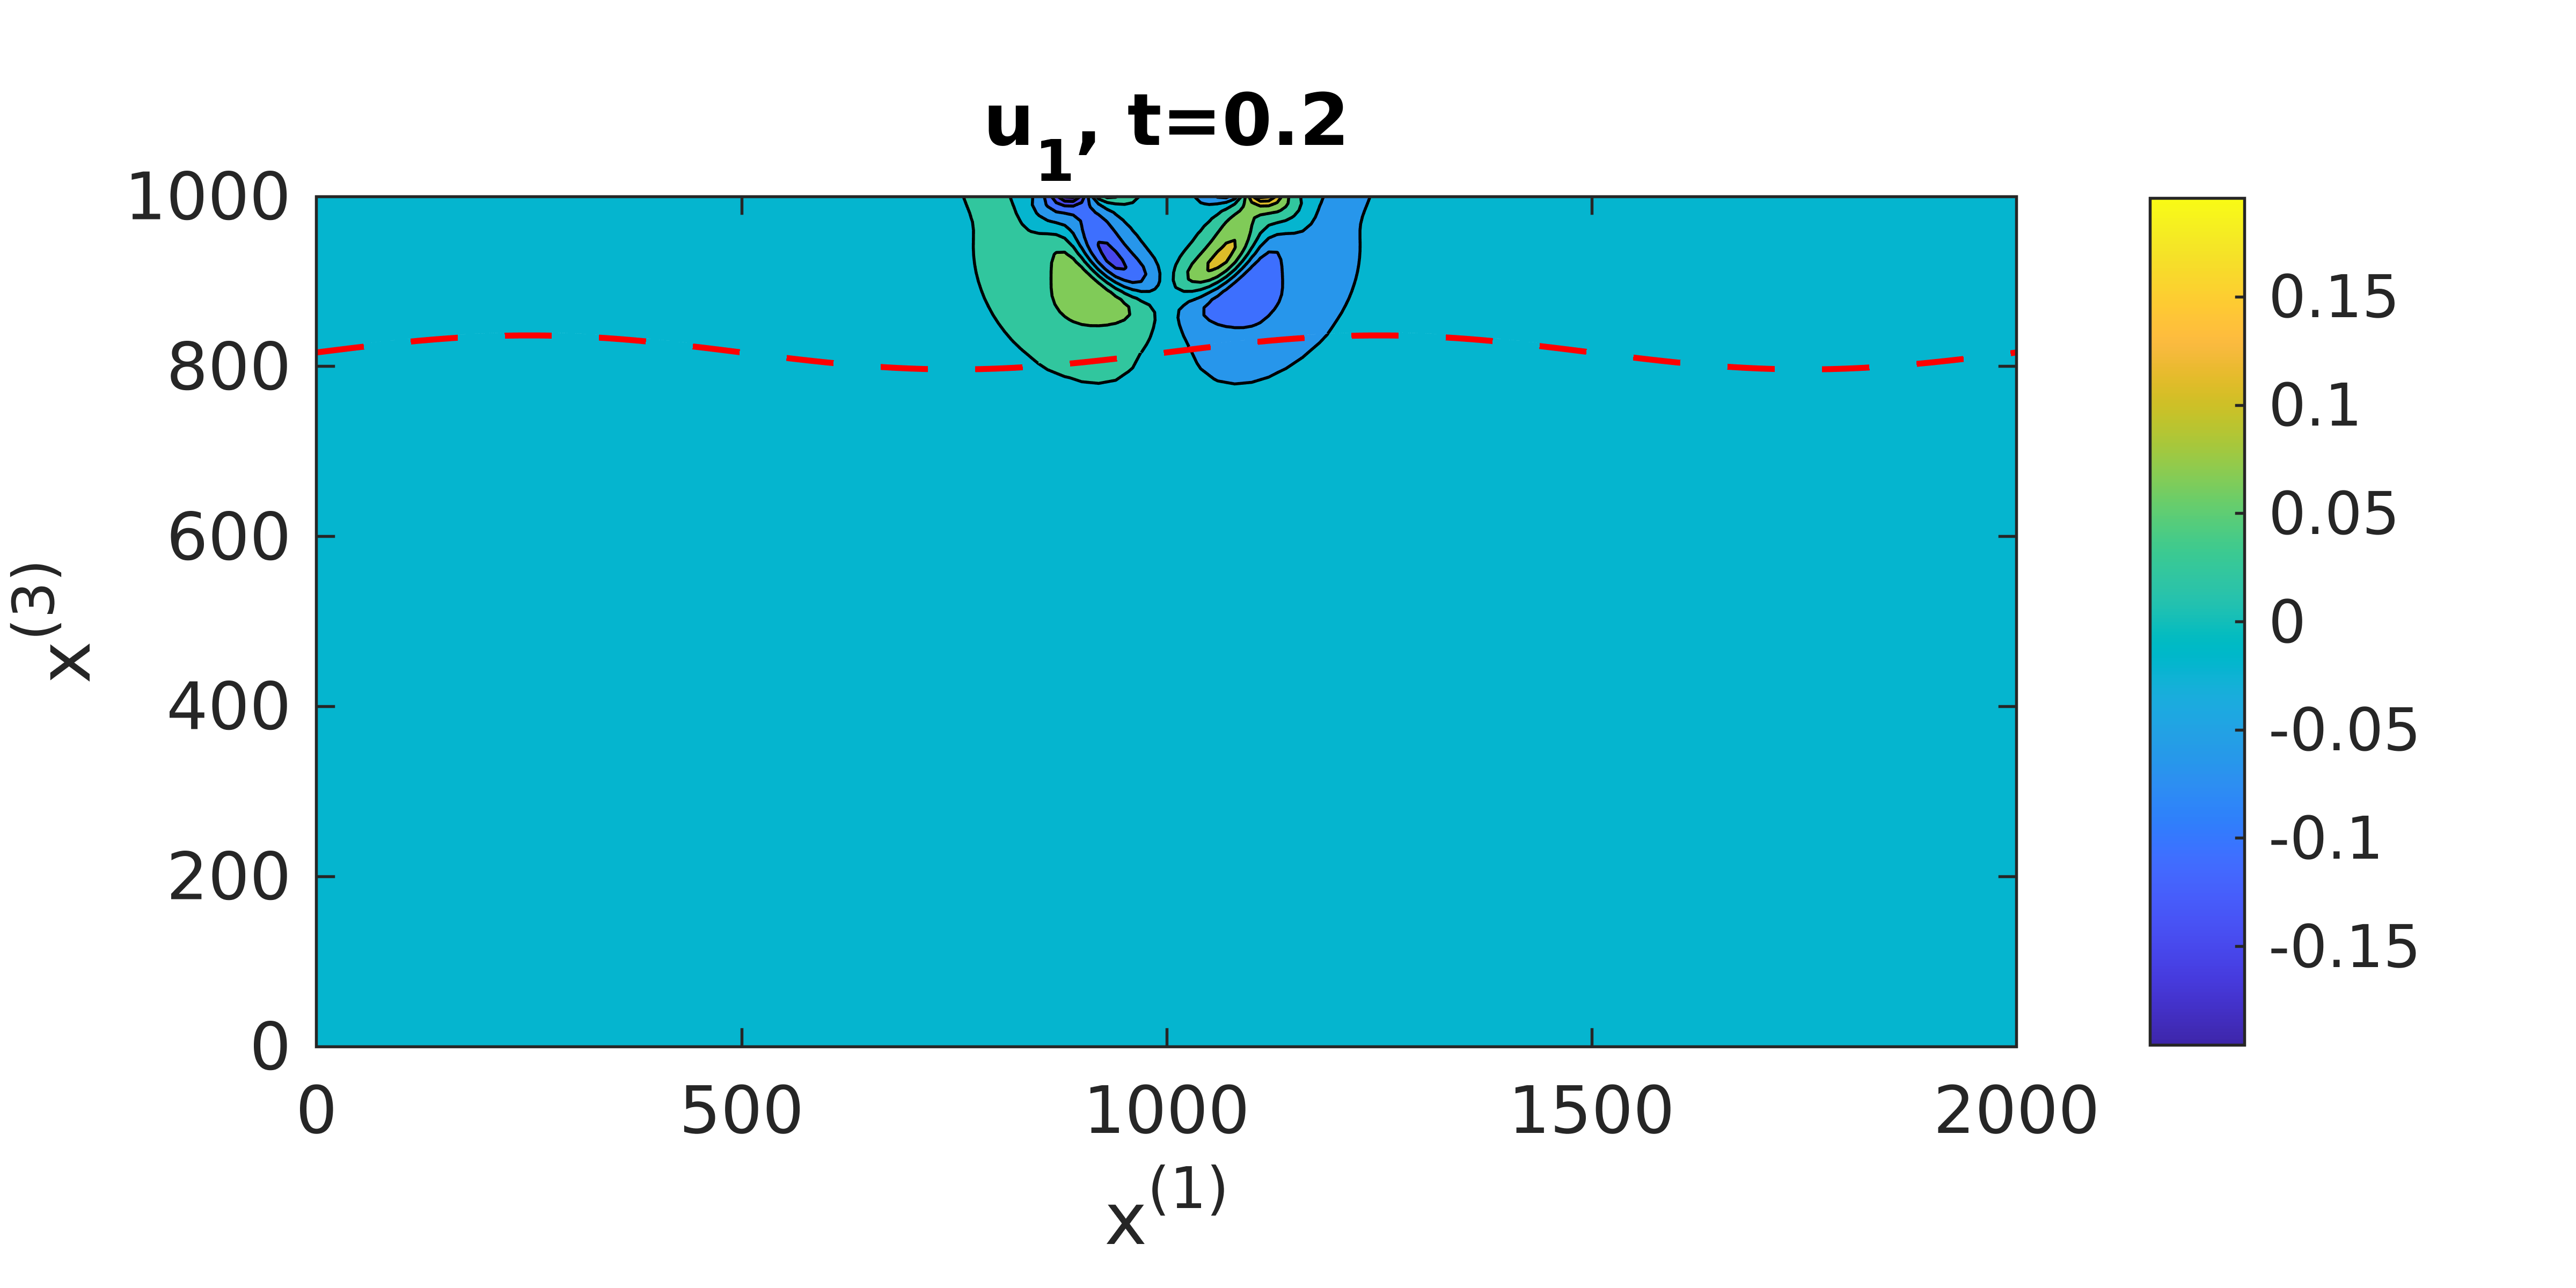
\includegraphics[width=0.49\textwidth,trim={0.05cm 0.1cm 0.55cm 0.45cm}, clip]{u1_t02_curvi.png}
	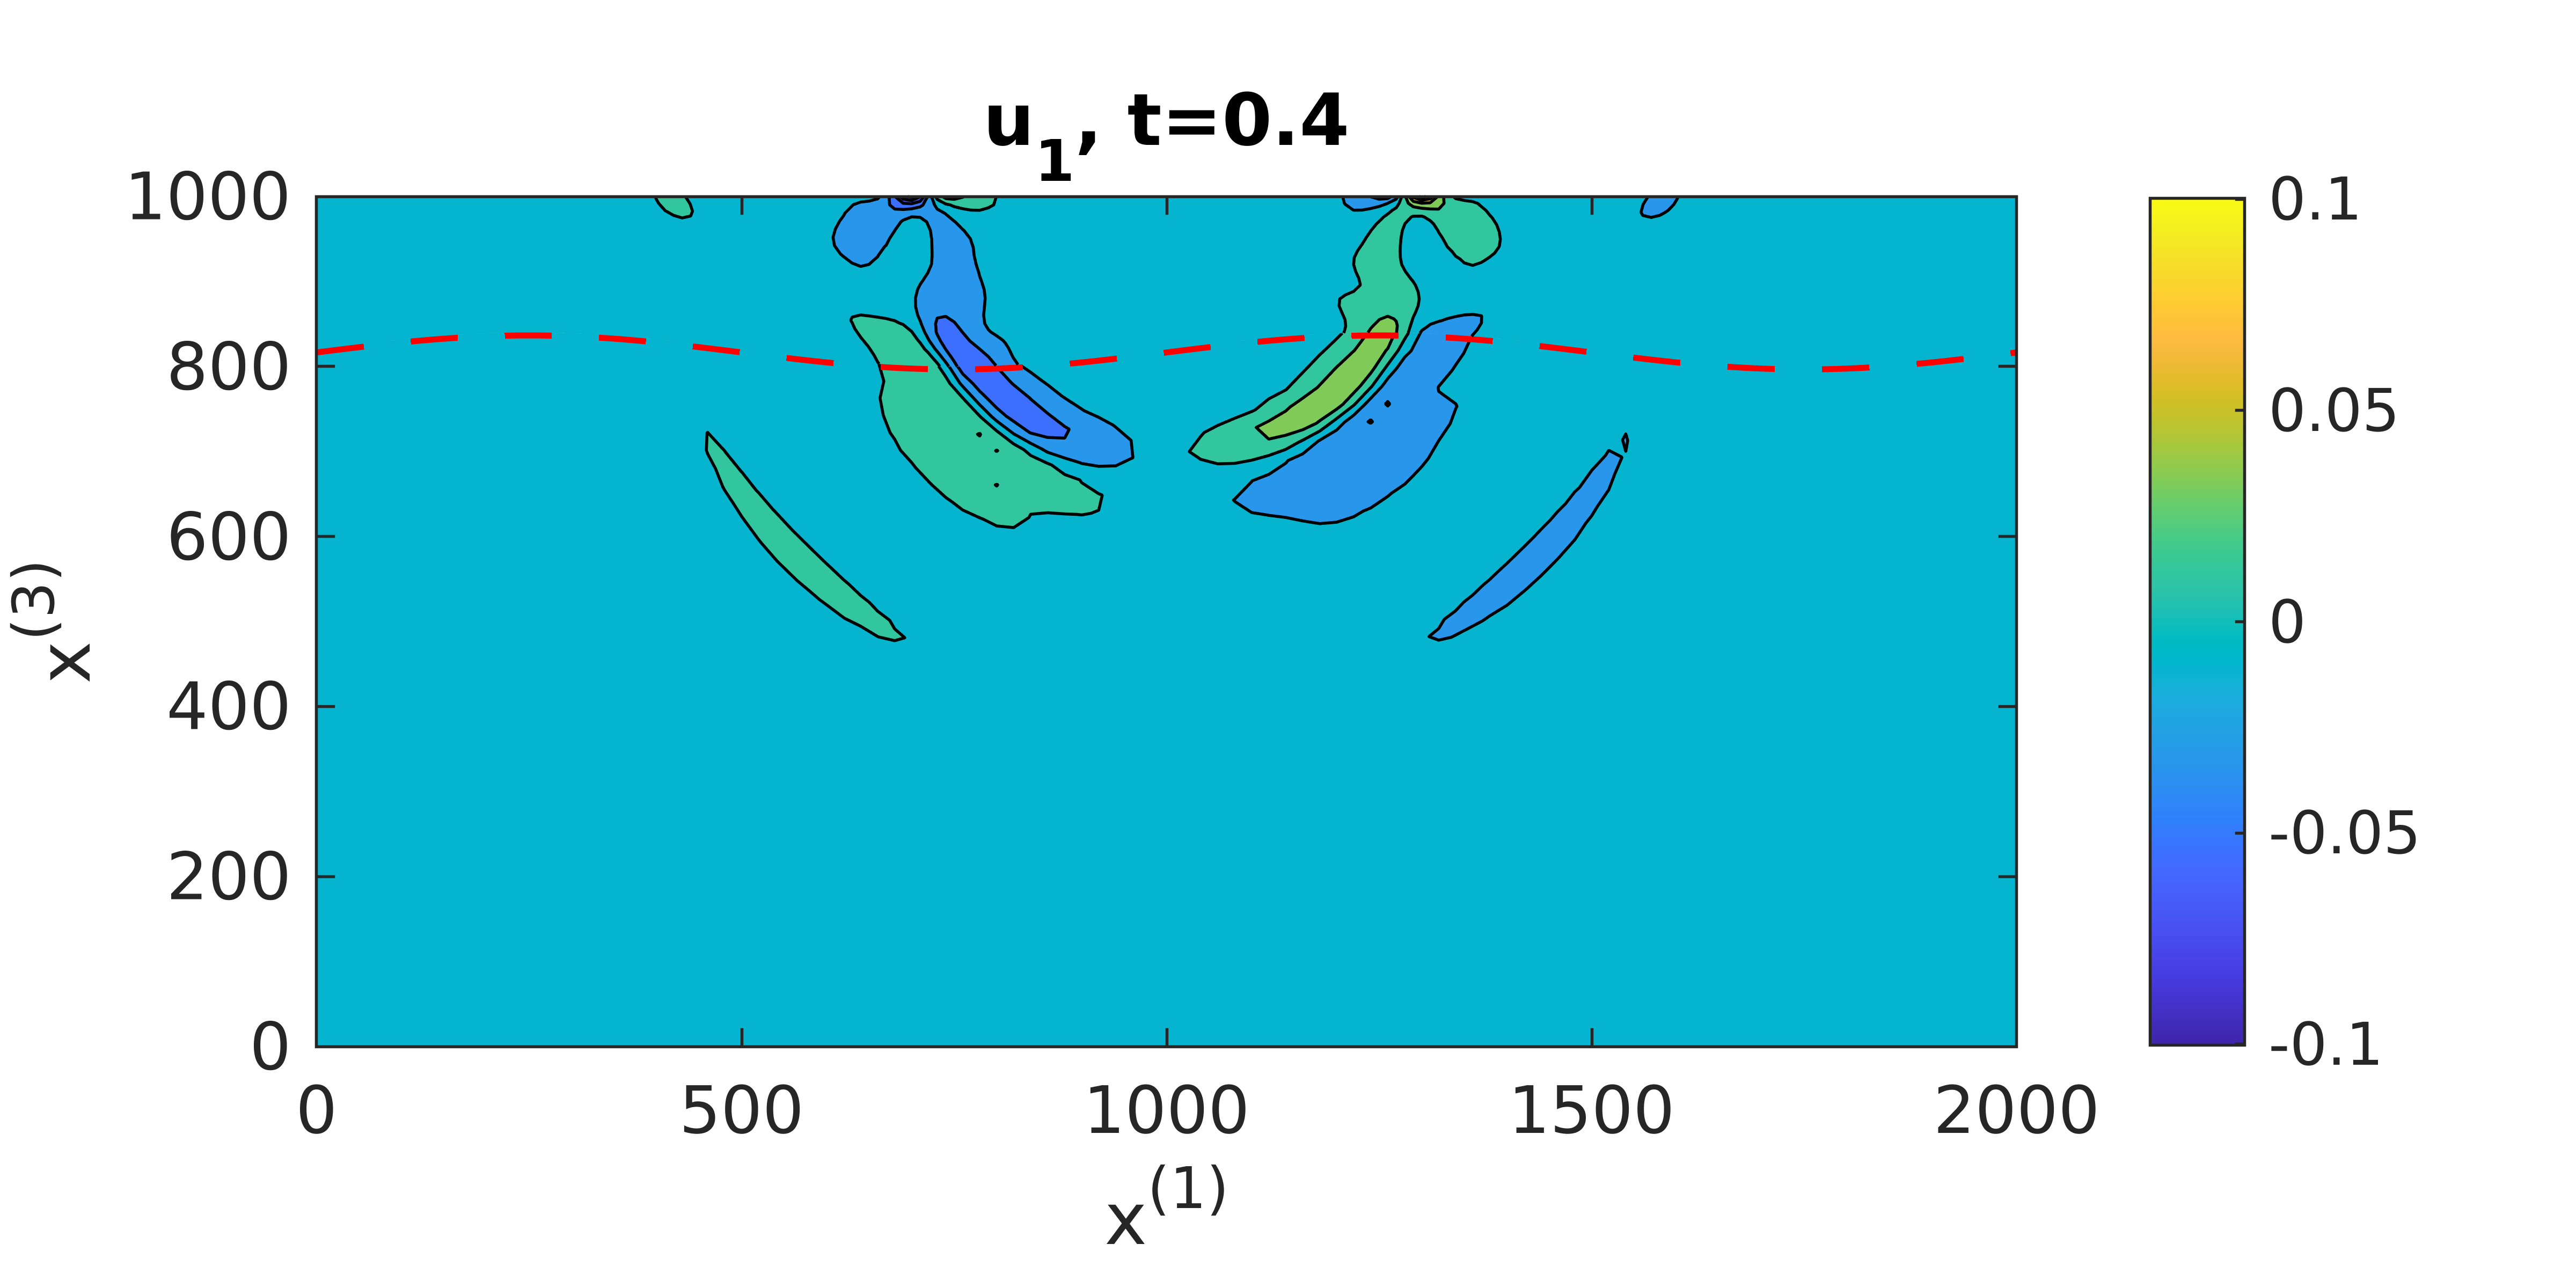
\includegraphics[width=0.49\textwidth,trim={0.05cm 0.1cm 0.55cm 0.45cm}, clip]{u1_t04_curvi.png}\\
	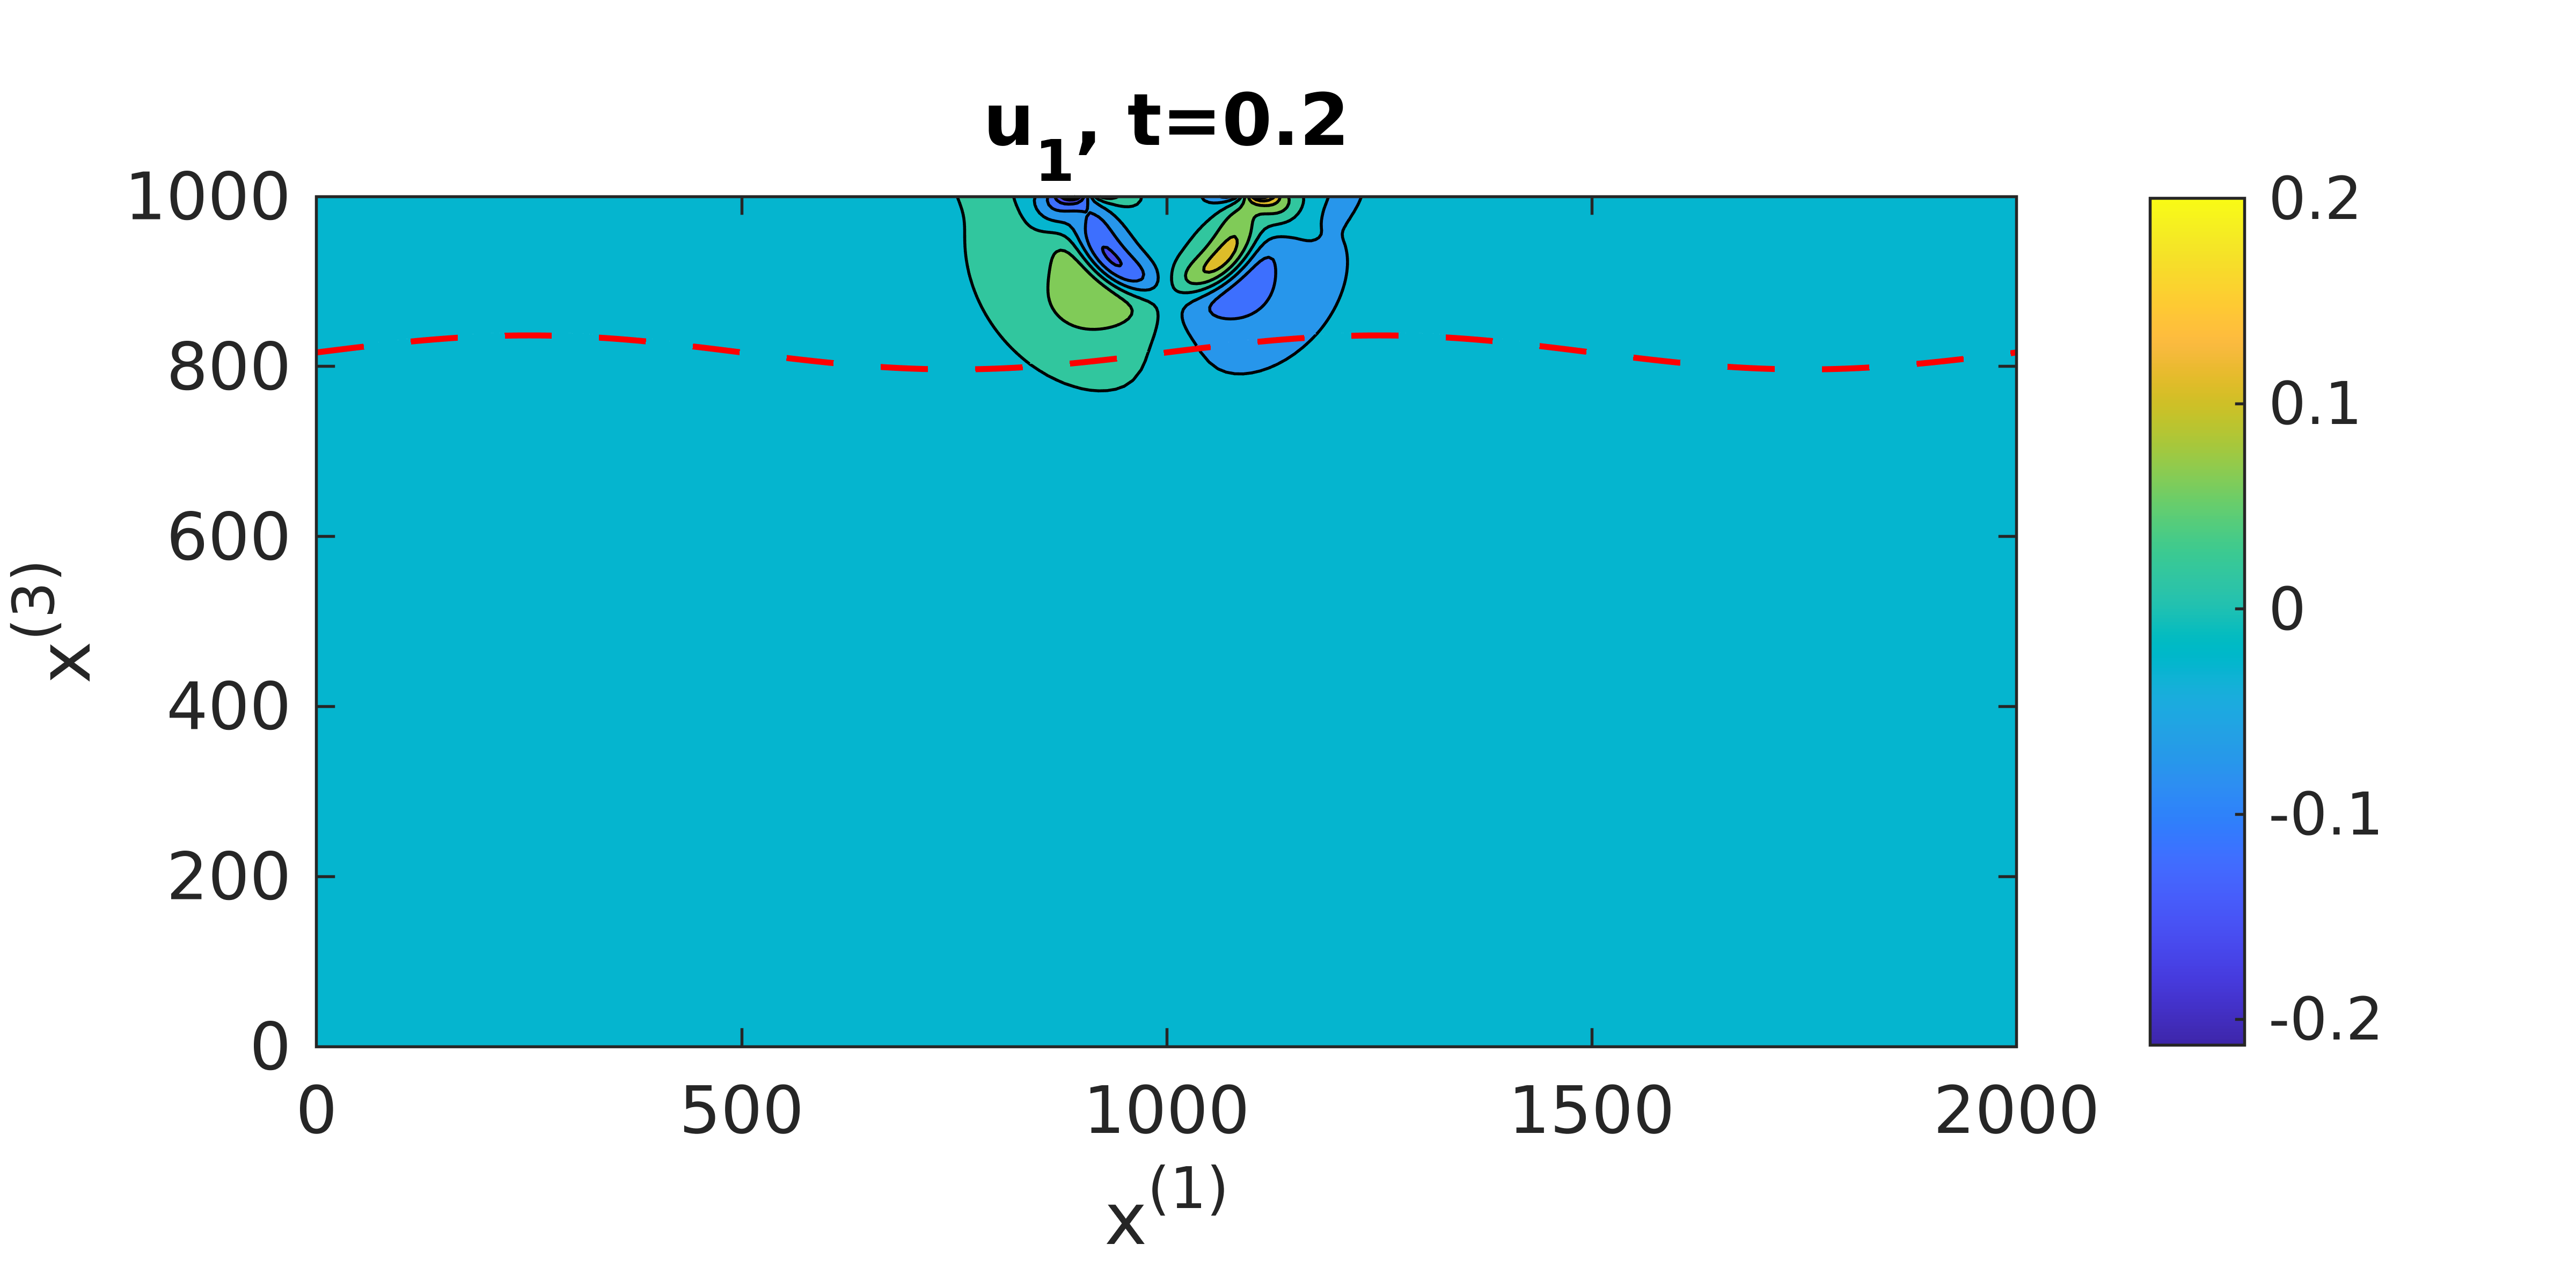
\includegraphics[width=0.49\textwidth,trim={0.05cm 0.1cm 0.55cm 0.45cm}, clip]{u1_t02_curvi_finer.png}
	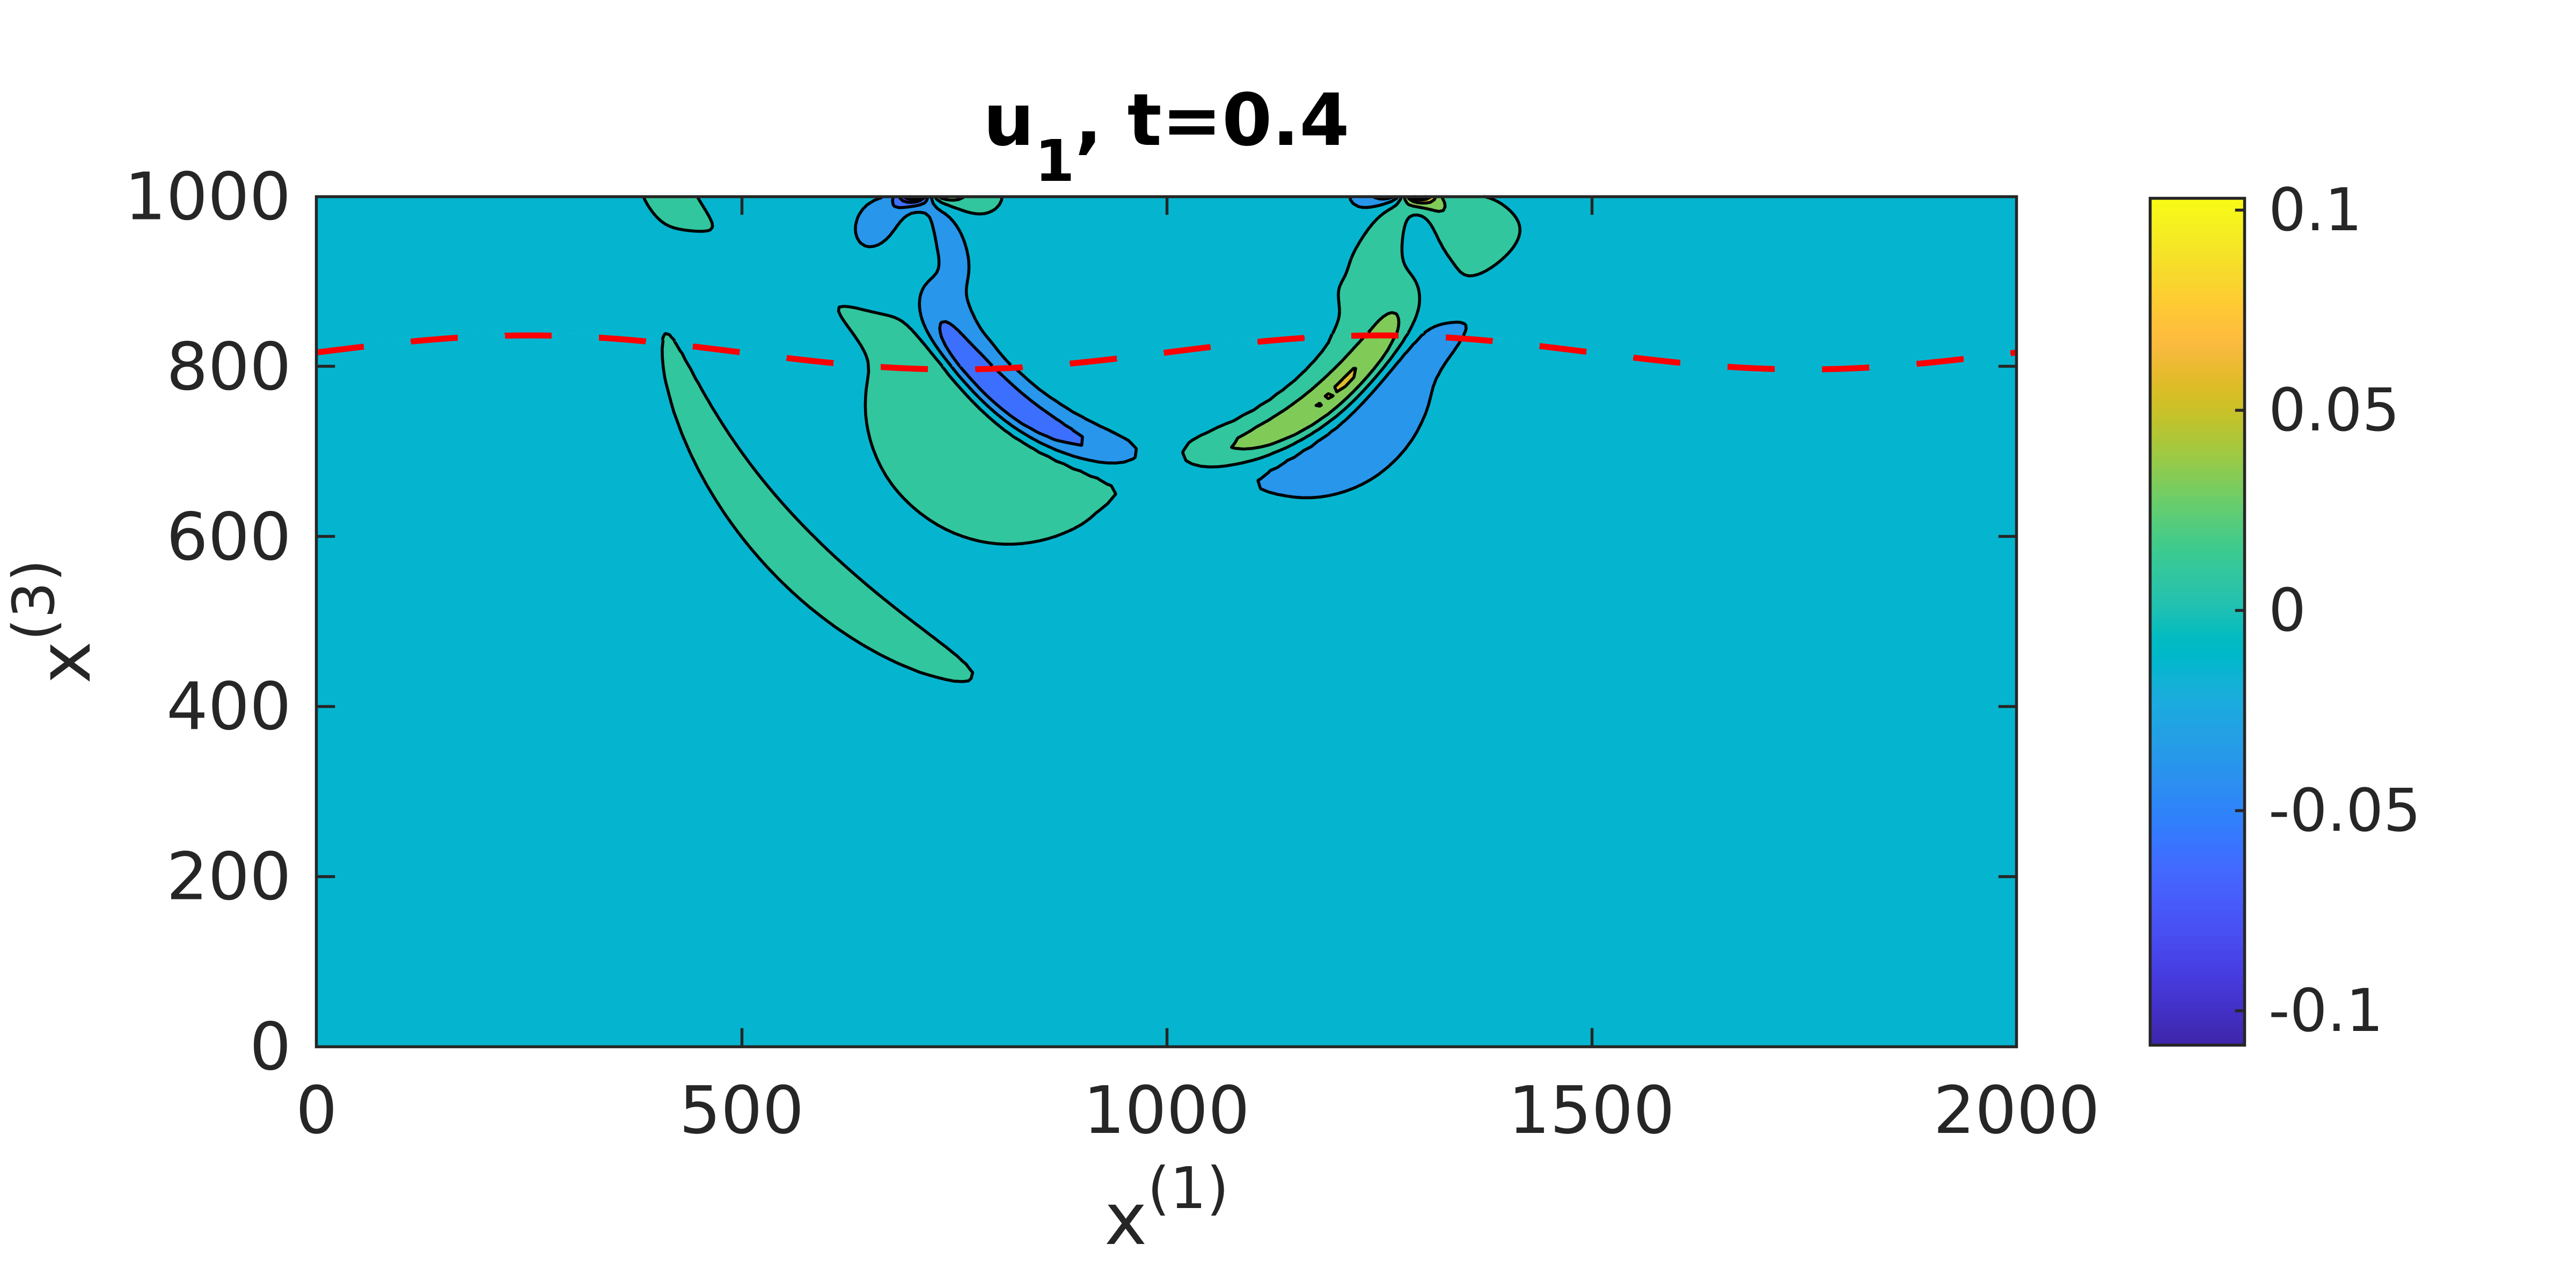
\includegraphics[width=0.49\textwidth,trim={0.05cm 0.1cm 0.55cm 0.45cm}, clip]{u1_t04_curvi_finer.png}
\caption{The graphs for $u_1$. In the top, middle and bottom panel, we show numerical solutions at $t=0.2$ and $t=0.4$ computed with Mesh 1, Mesh 2 and Mesh 3, respectively. The curved interfaces are marked with the red dash lines.}
\label{u1}
\end{figure}

%\begin{figure}[htbp]
%	\centering
%	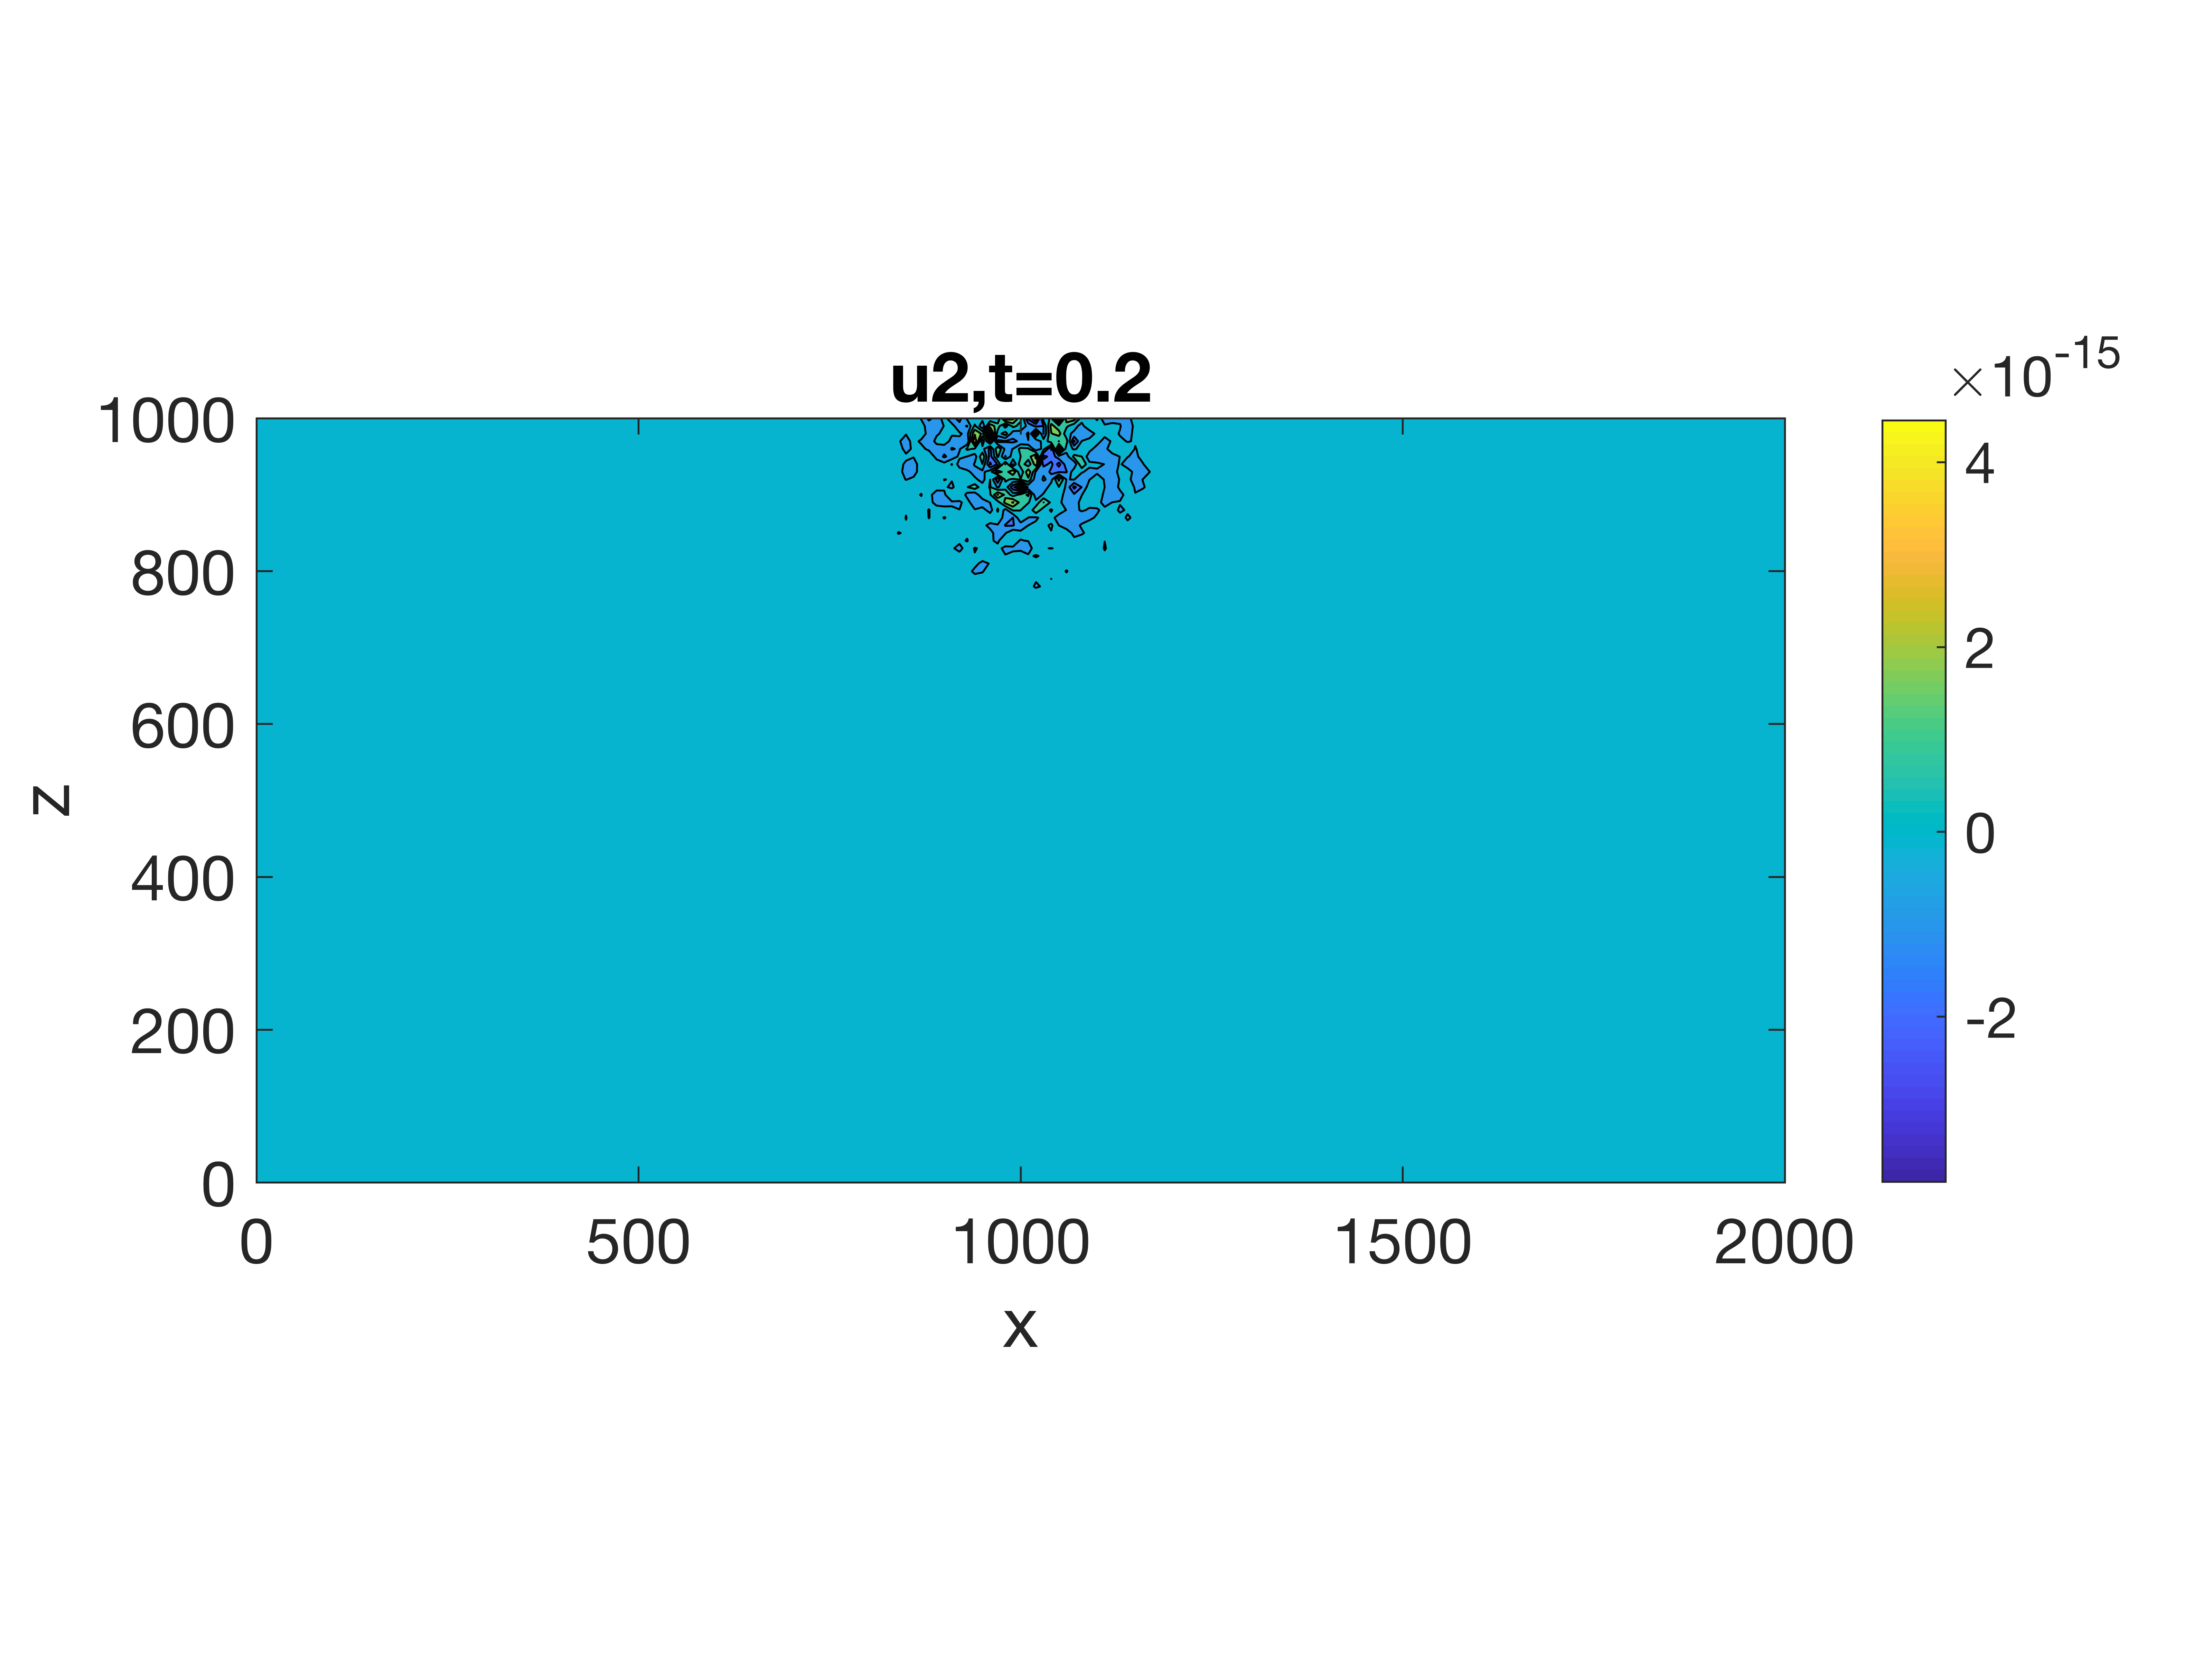
\includegraphics[width=0.4\textwidth,trim={0 2.8cm 0 2.8cm}, clip]{u2_t02_cartesian.png}
%	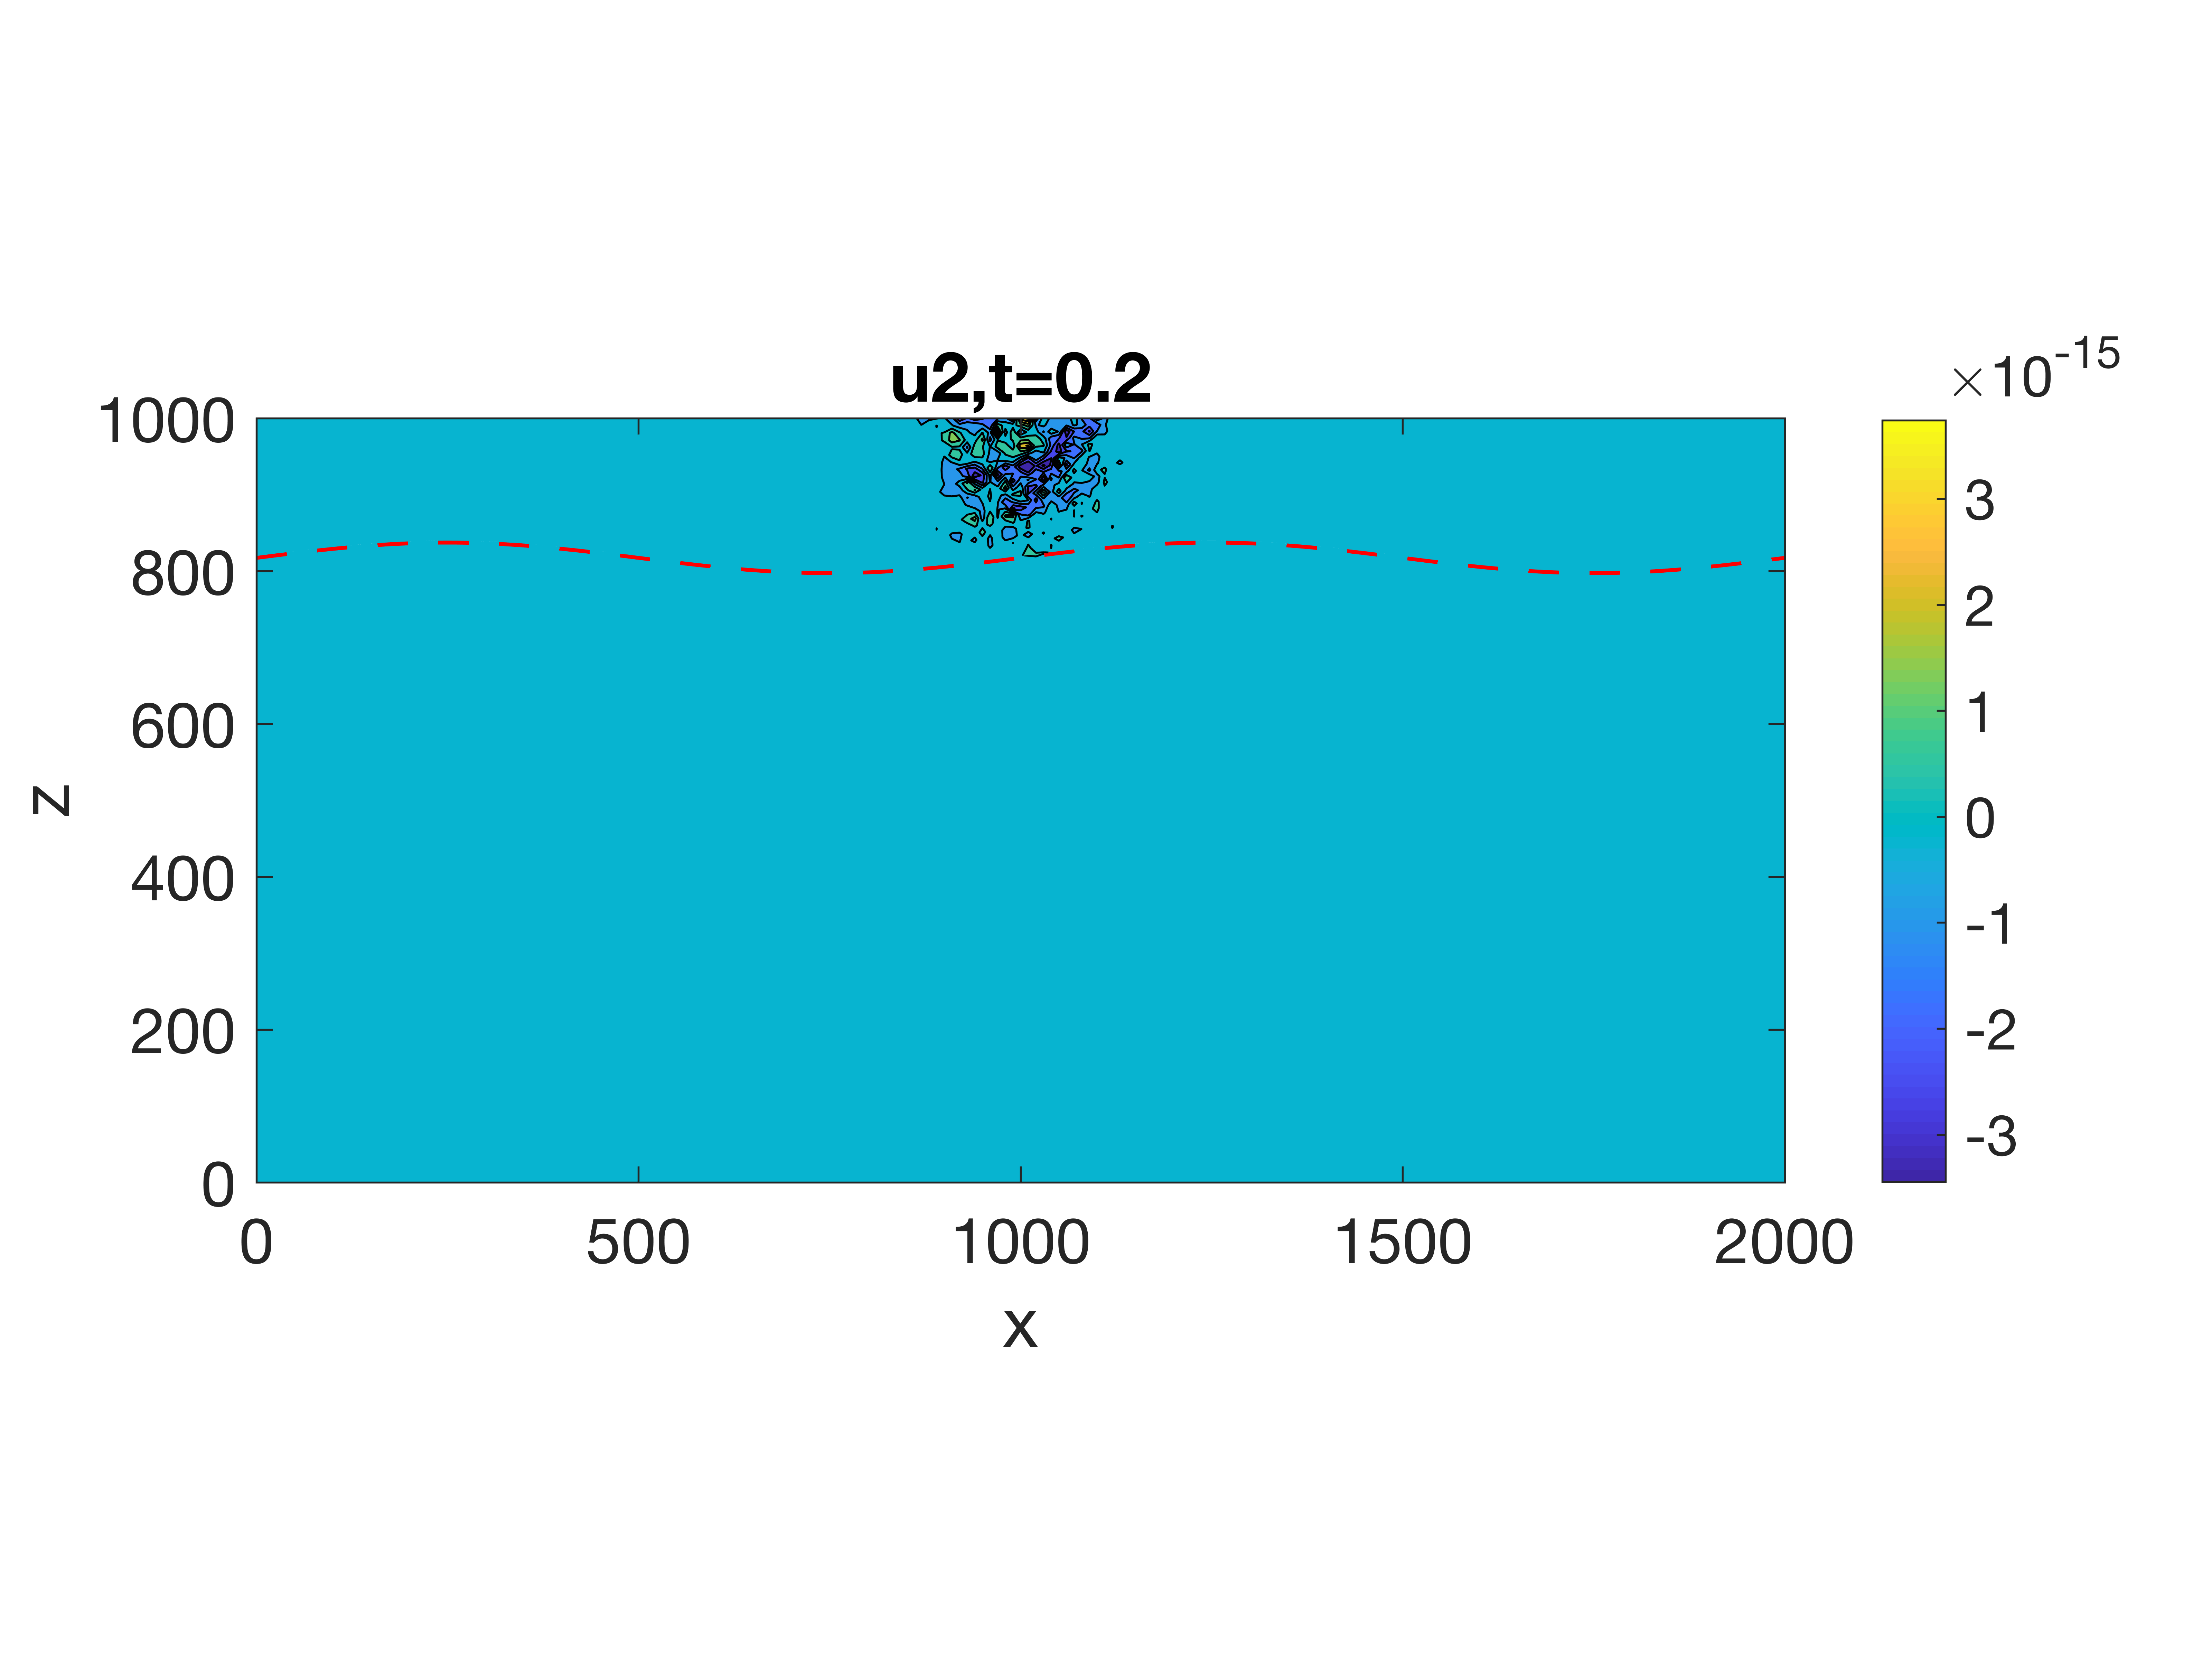
\includegraphics[width=0.4\textwidth,trim={0 2.8cm 0 2.8cm}, clip]{u2_t02_curvi_mr.png}\\
%	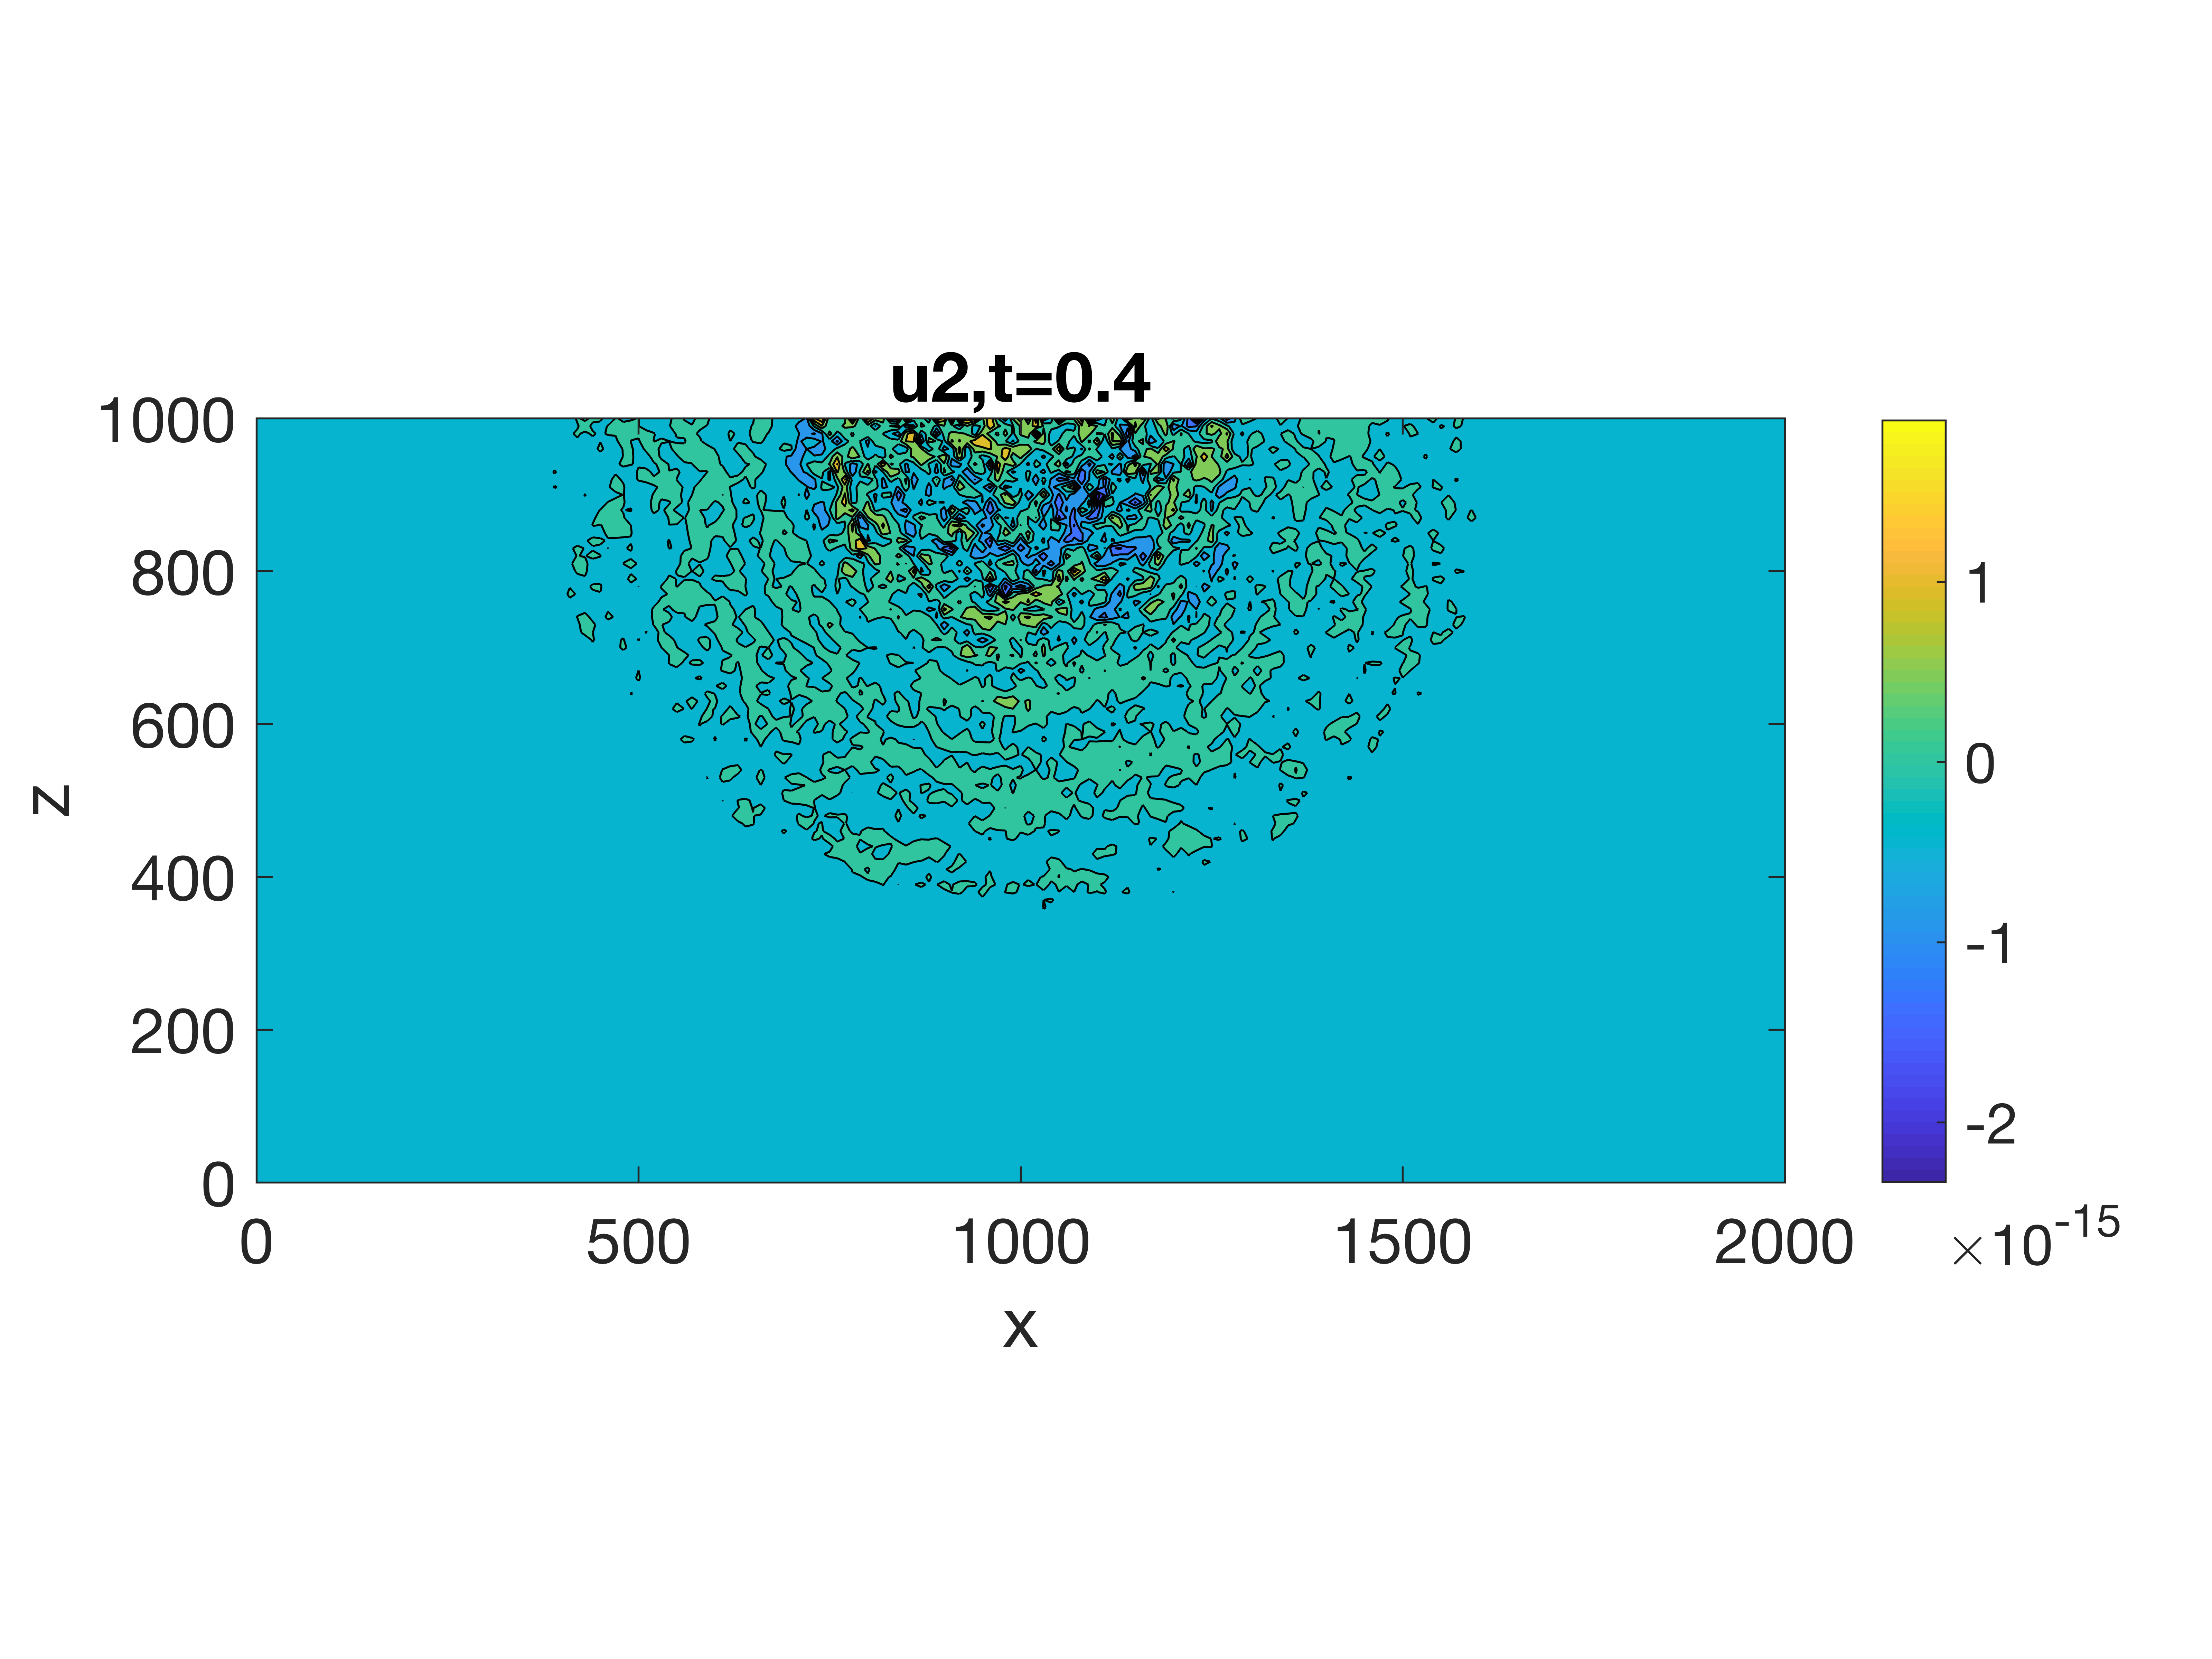
\includegraphics[width=0.4\textwidth,trim={0 2.8cm 0 2.8cm}, clip]{u2_t04_cartesian.png}
%	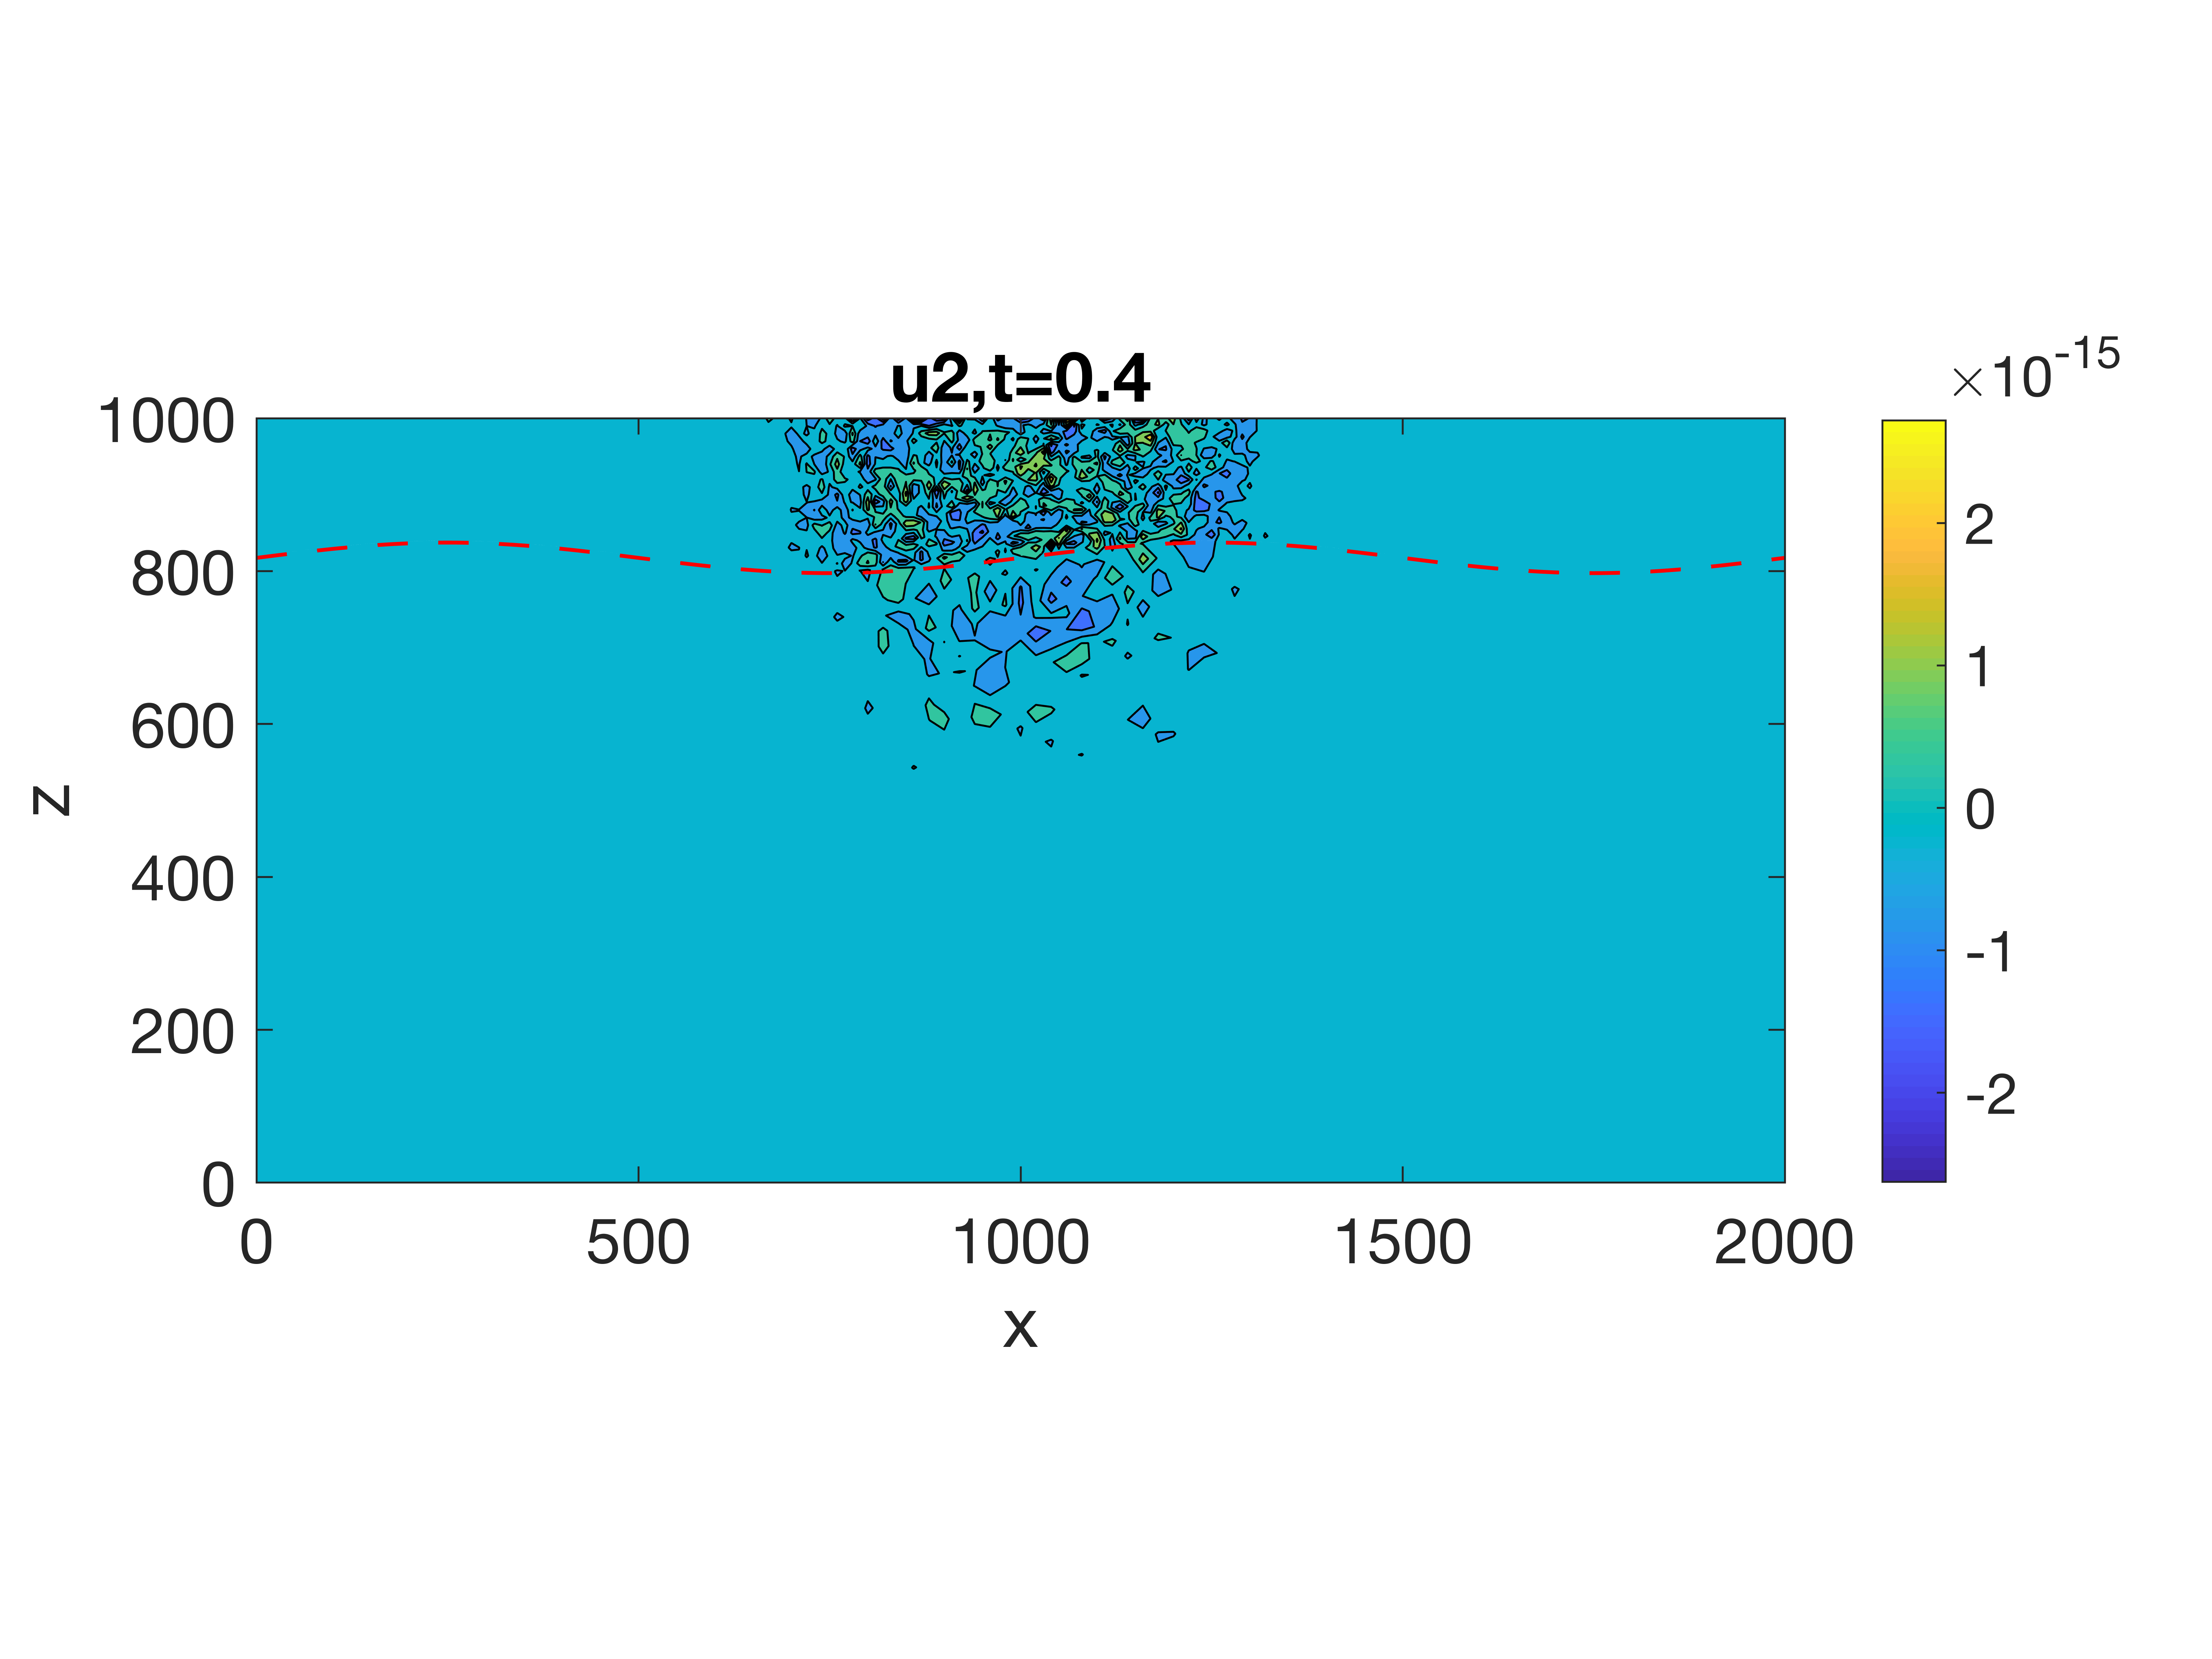
\includegraphics[width=0.4\textwidth,trim={0 2.8cm 0 2.8cm}, clip]{u2_t04_curvi_mr.png}
%	\caption{The graph for $u_2$. From left to right are for Cartesian mesh without mesh refinement interface and curvilinear mesh with mesh refinement interface respectively. From top to bottom are for $t = 0.2$ and $t = 0.4$ respectively. Note that $x,z$ in the graph correspond to $x^{(1)}, x^{(3)}$ respectively.}\label{u2}
%\end{figure}

\begin{figure}[htbp]
	\centering
	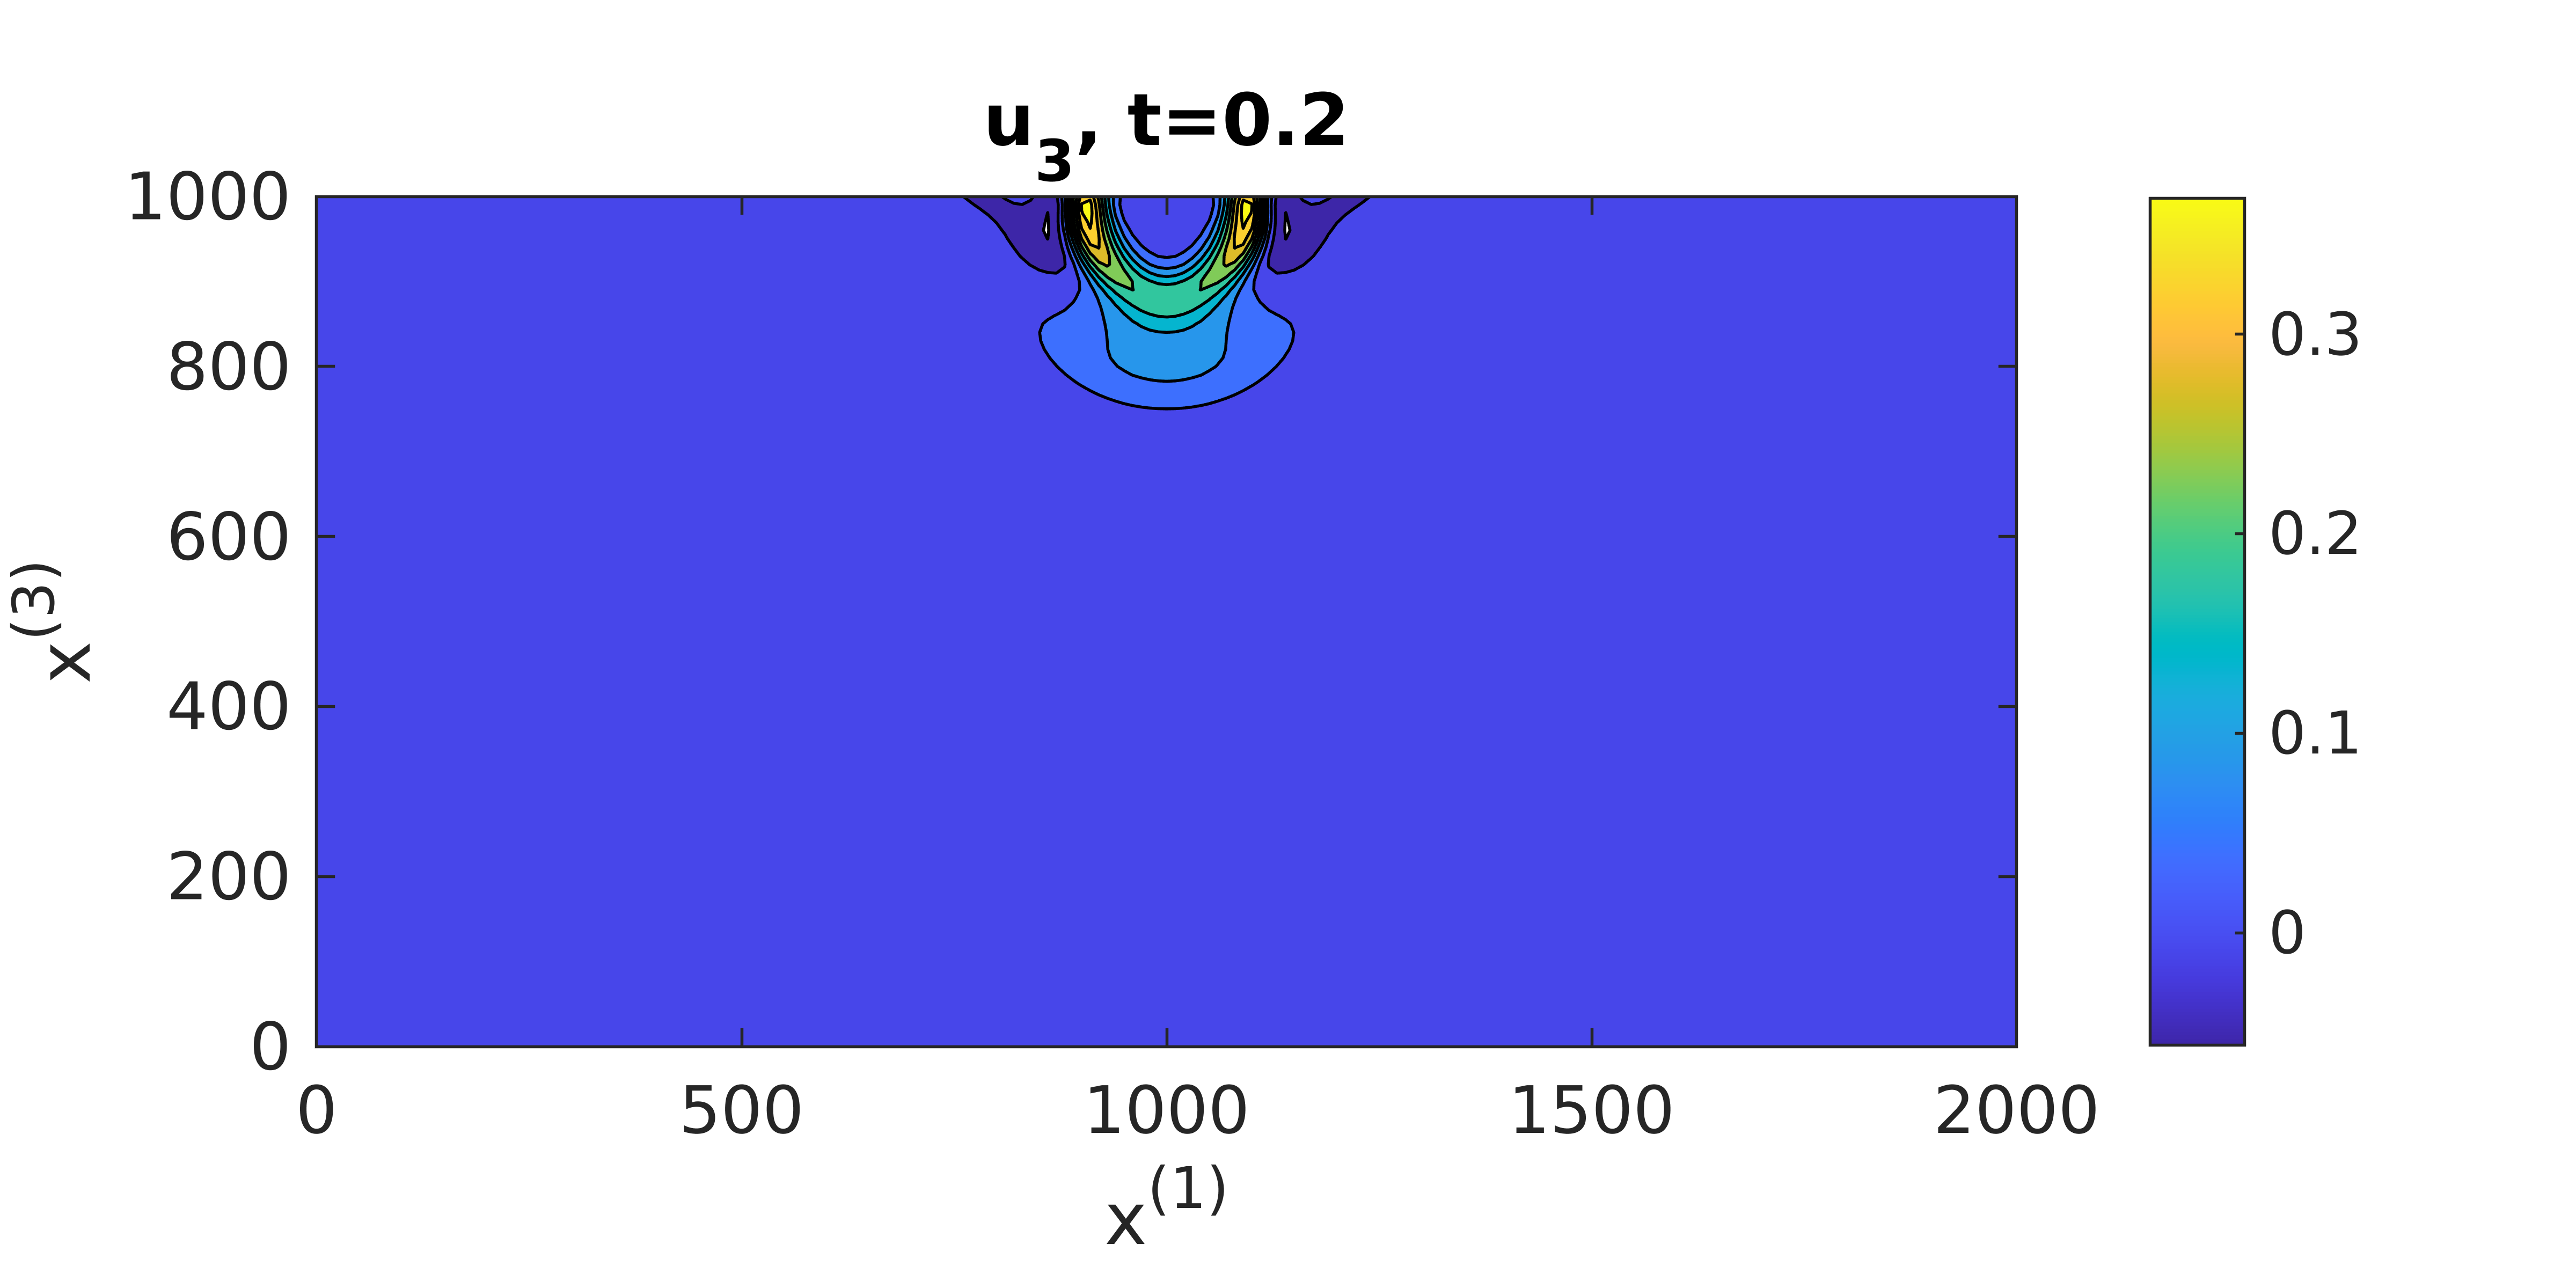
\includegraphics[width=0.49\textwidth,trim={0.05cm 0.1cm 0.55cm 0.45cm}, clip]{u3_t02_cartesian.png}
	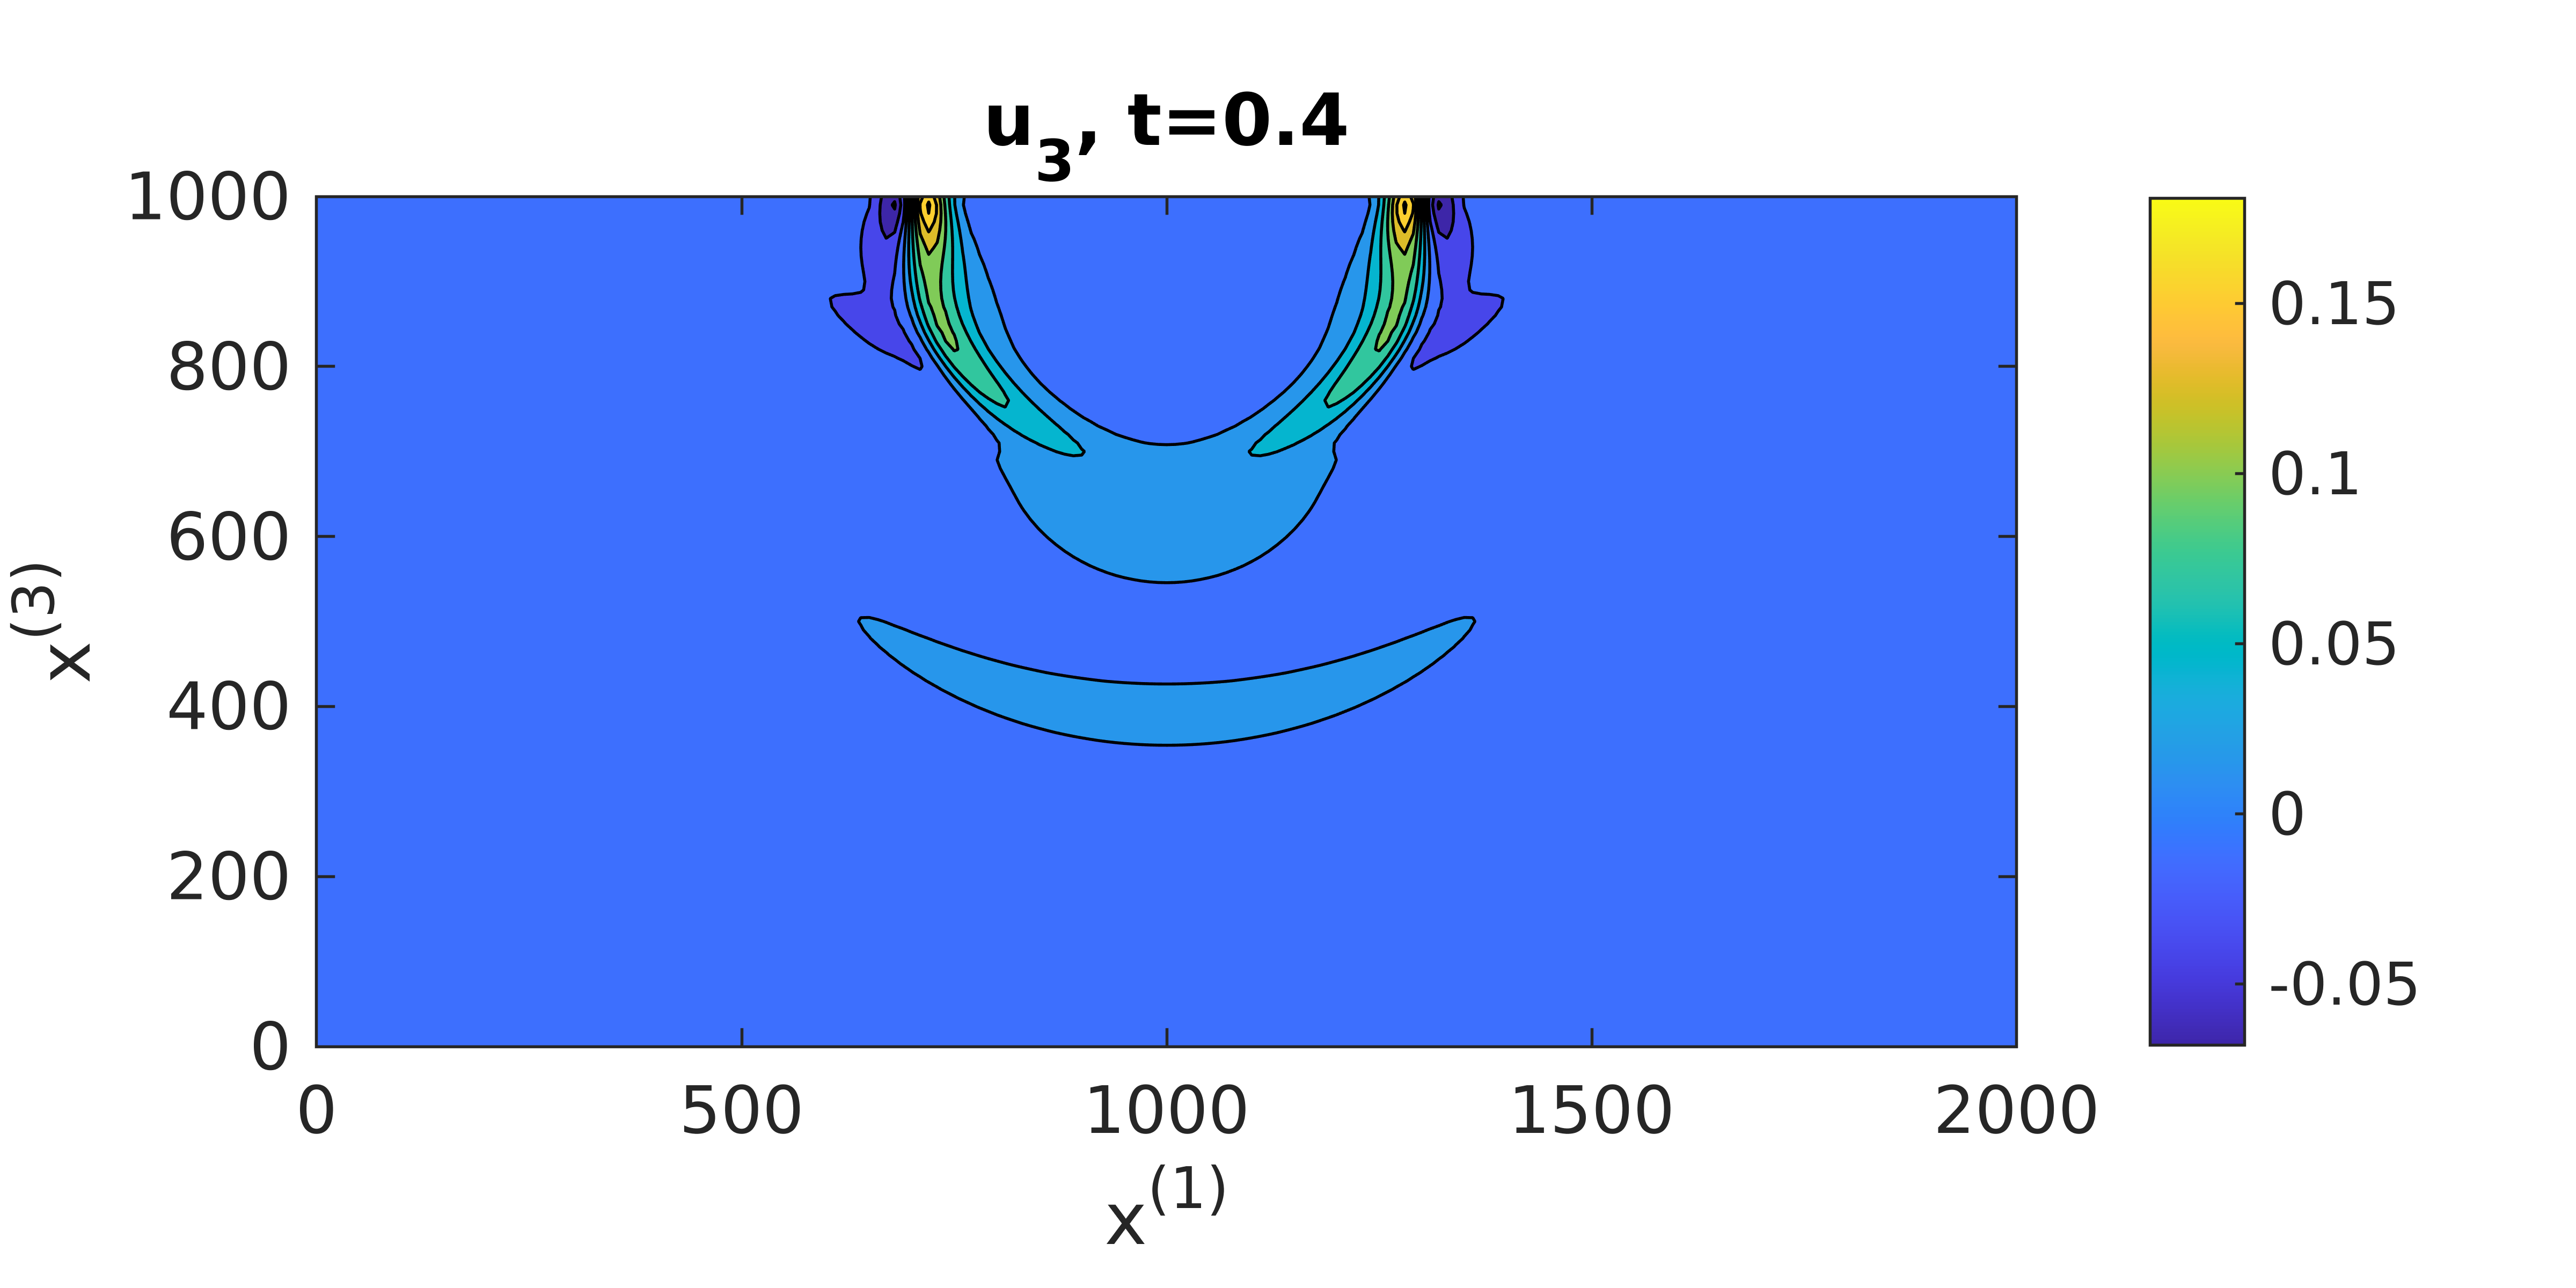
\includegraphics[width=0.49\textwidth,trim={0.05cm 0.1cm 0.55cm 0.45cm}, clip]{u3_t04_cartesian.png}\\
	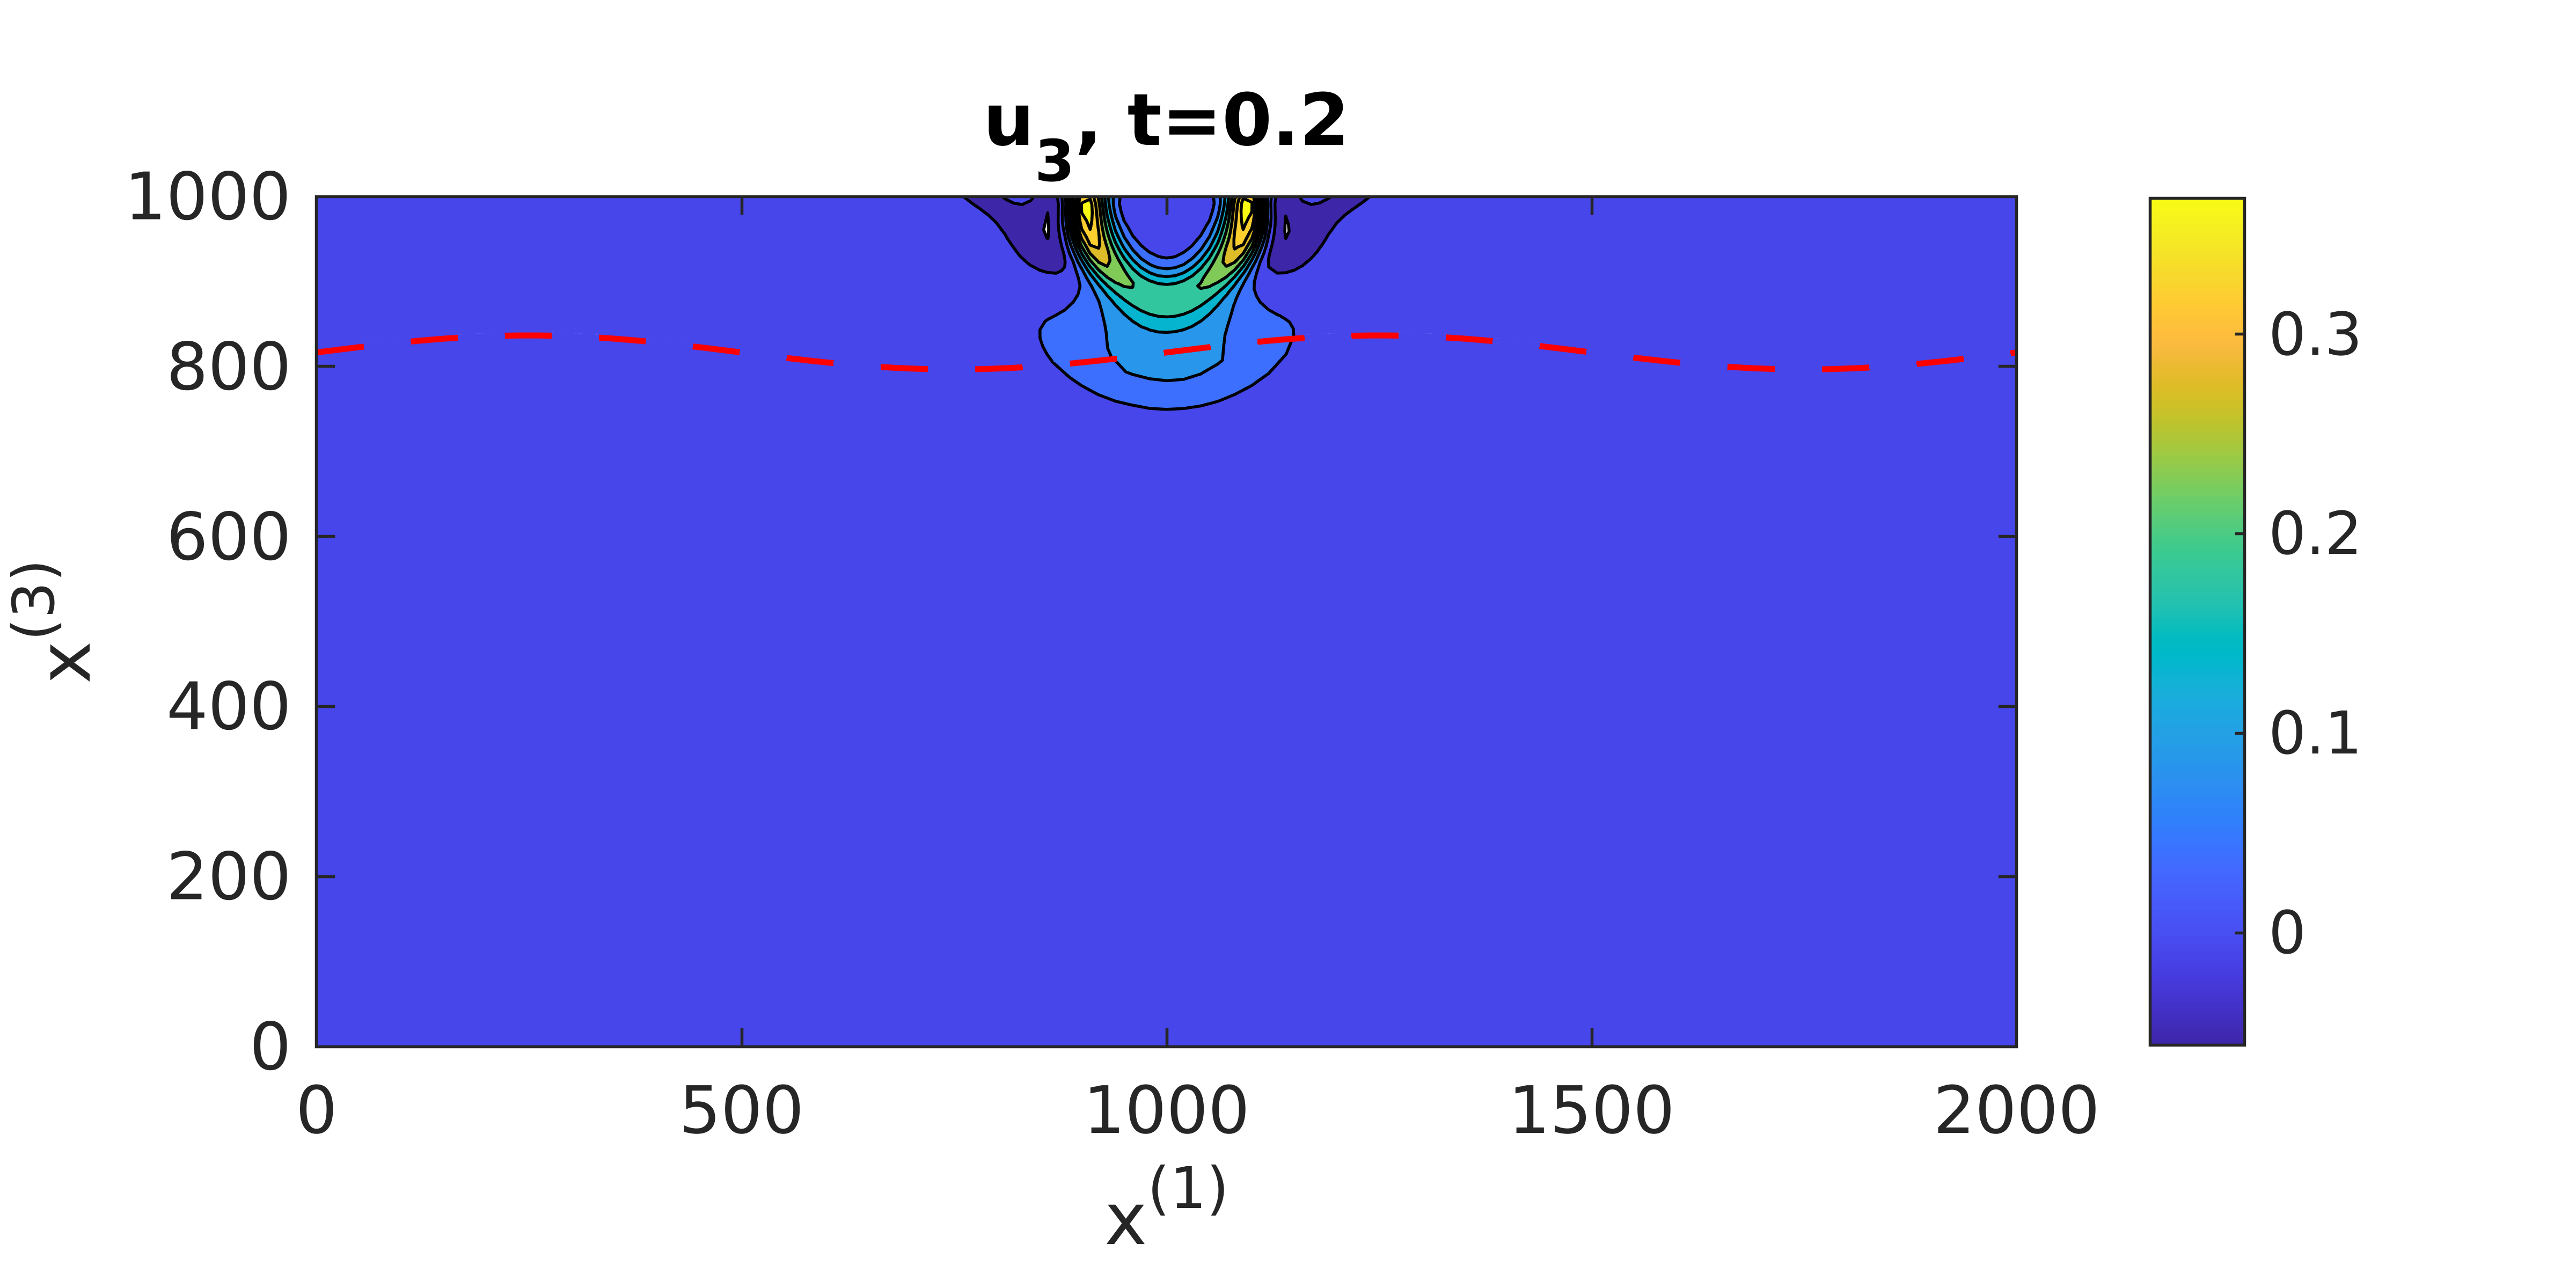
\includegraphics[width=0.49\textwidth,trim={0.05cm 0.1cm 0.55cm 0.45cm}, clip]{u3_t02_curvi.png}
	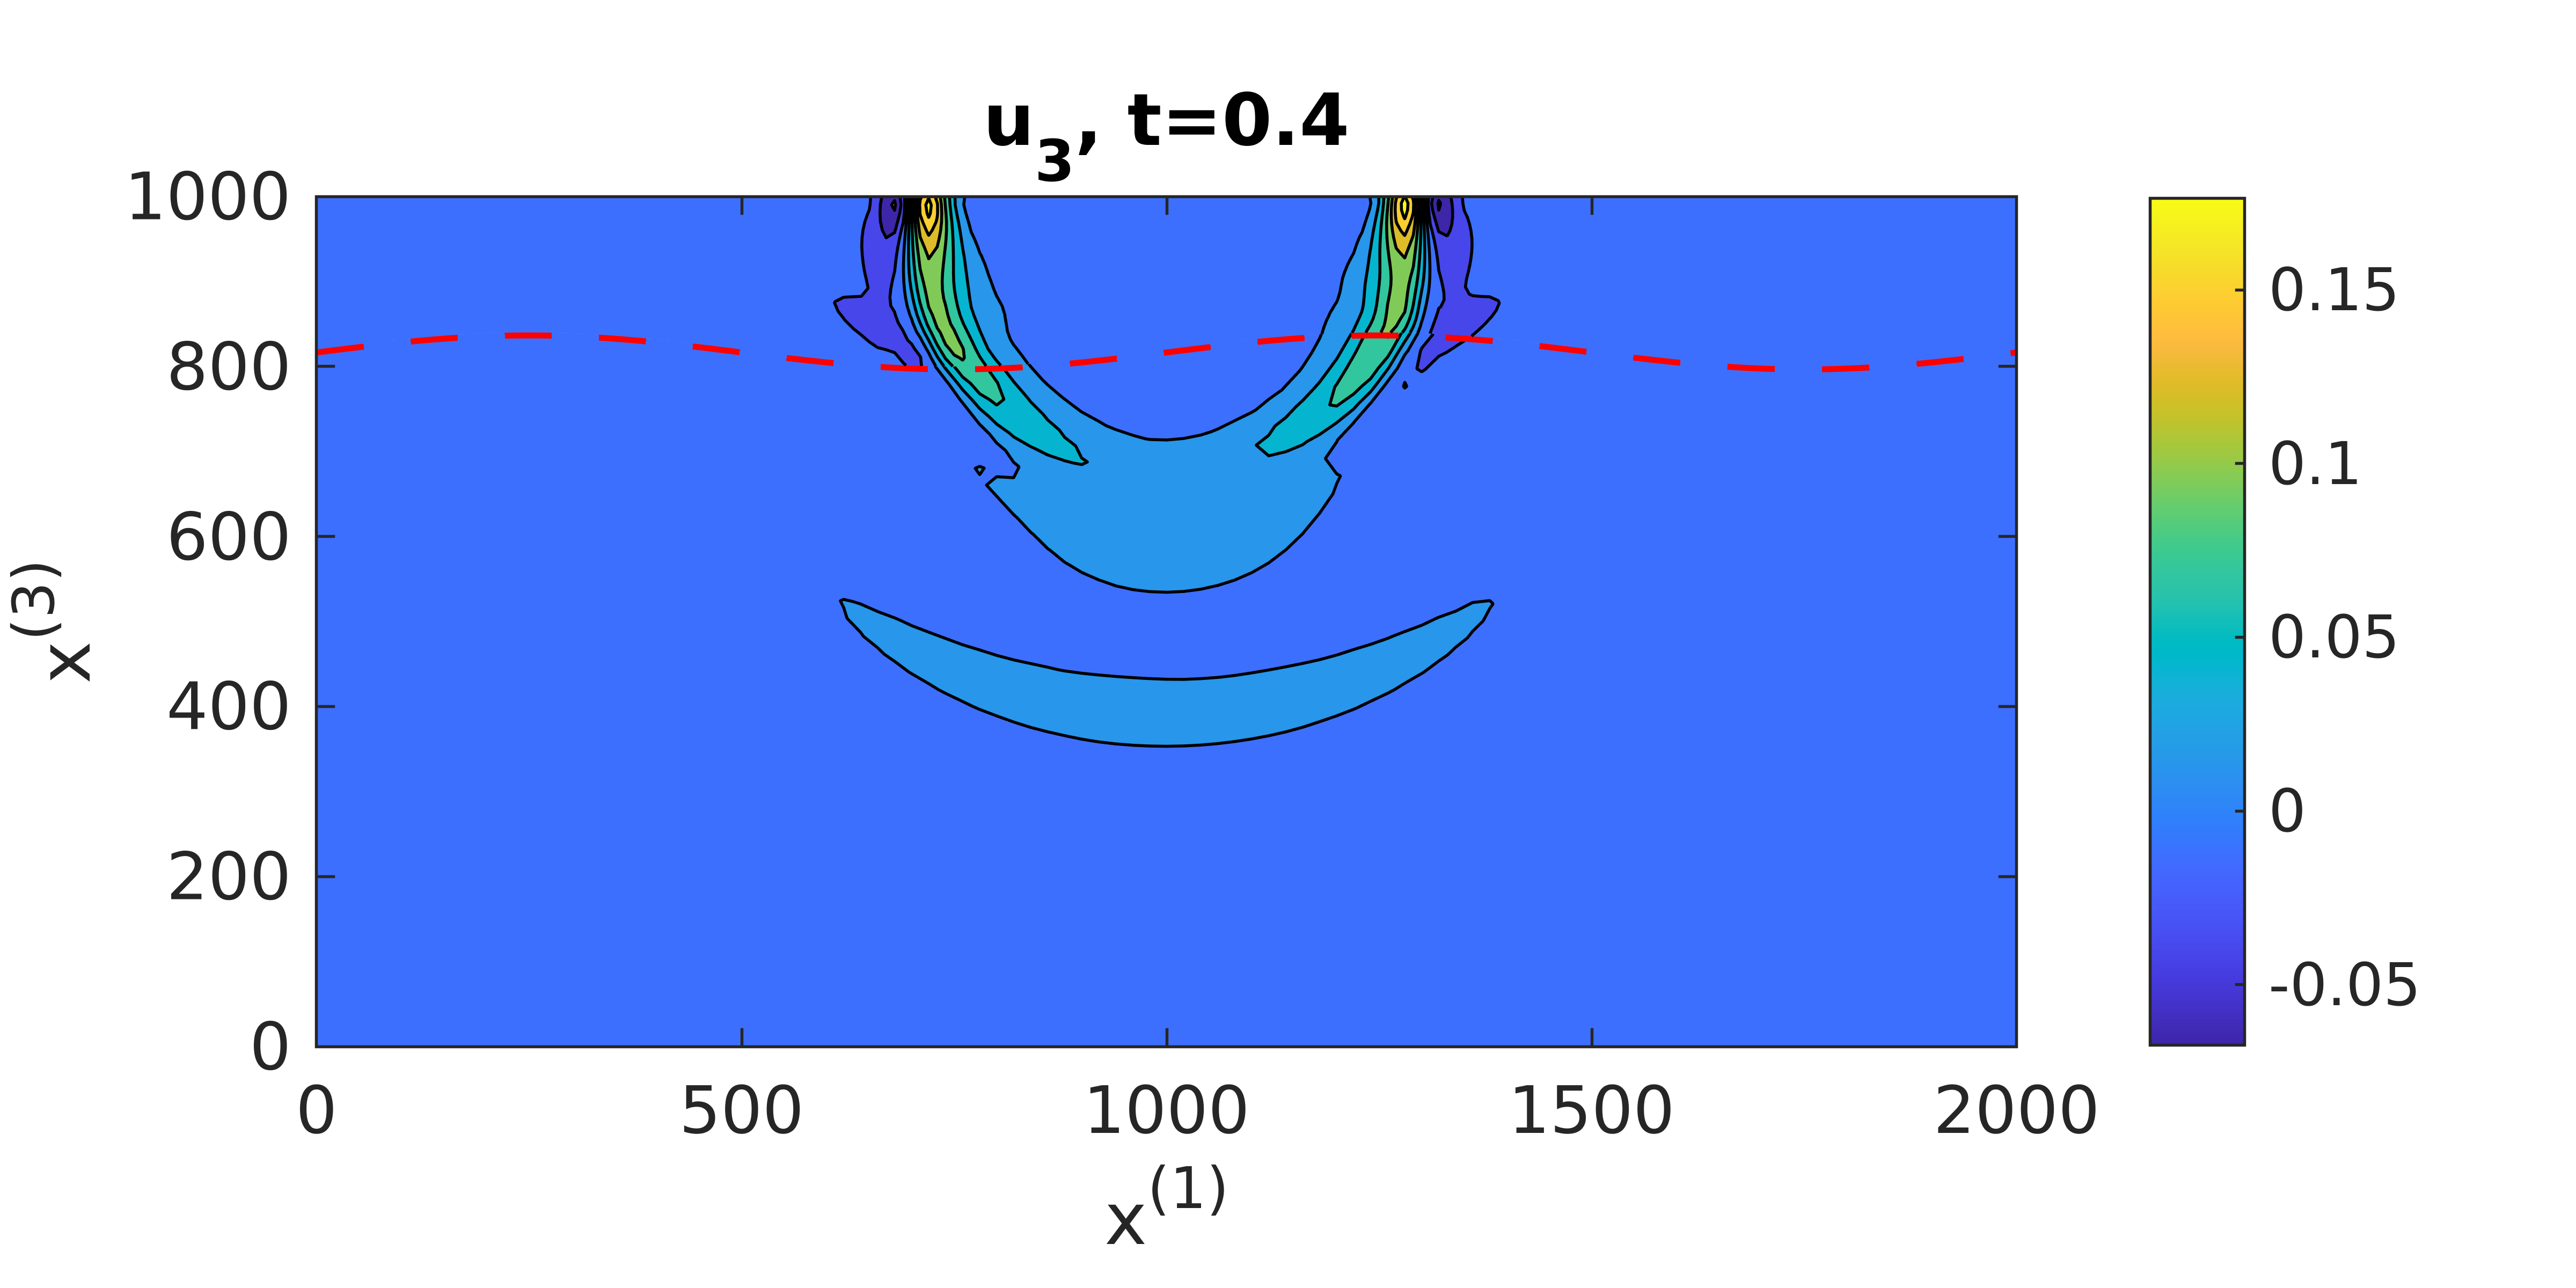
\includegraphics[width=0.49\textwidth,trim={0.05cm 0.1cm 0.55cm 0.45cm}, clip]{u3_t04_curvi.png}\\
	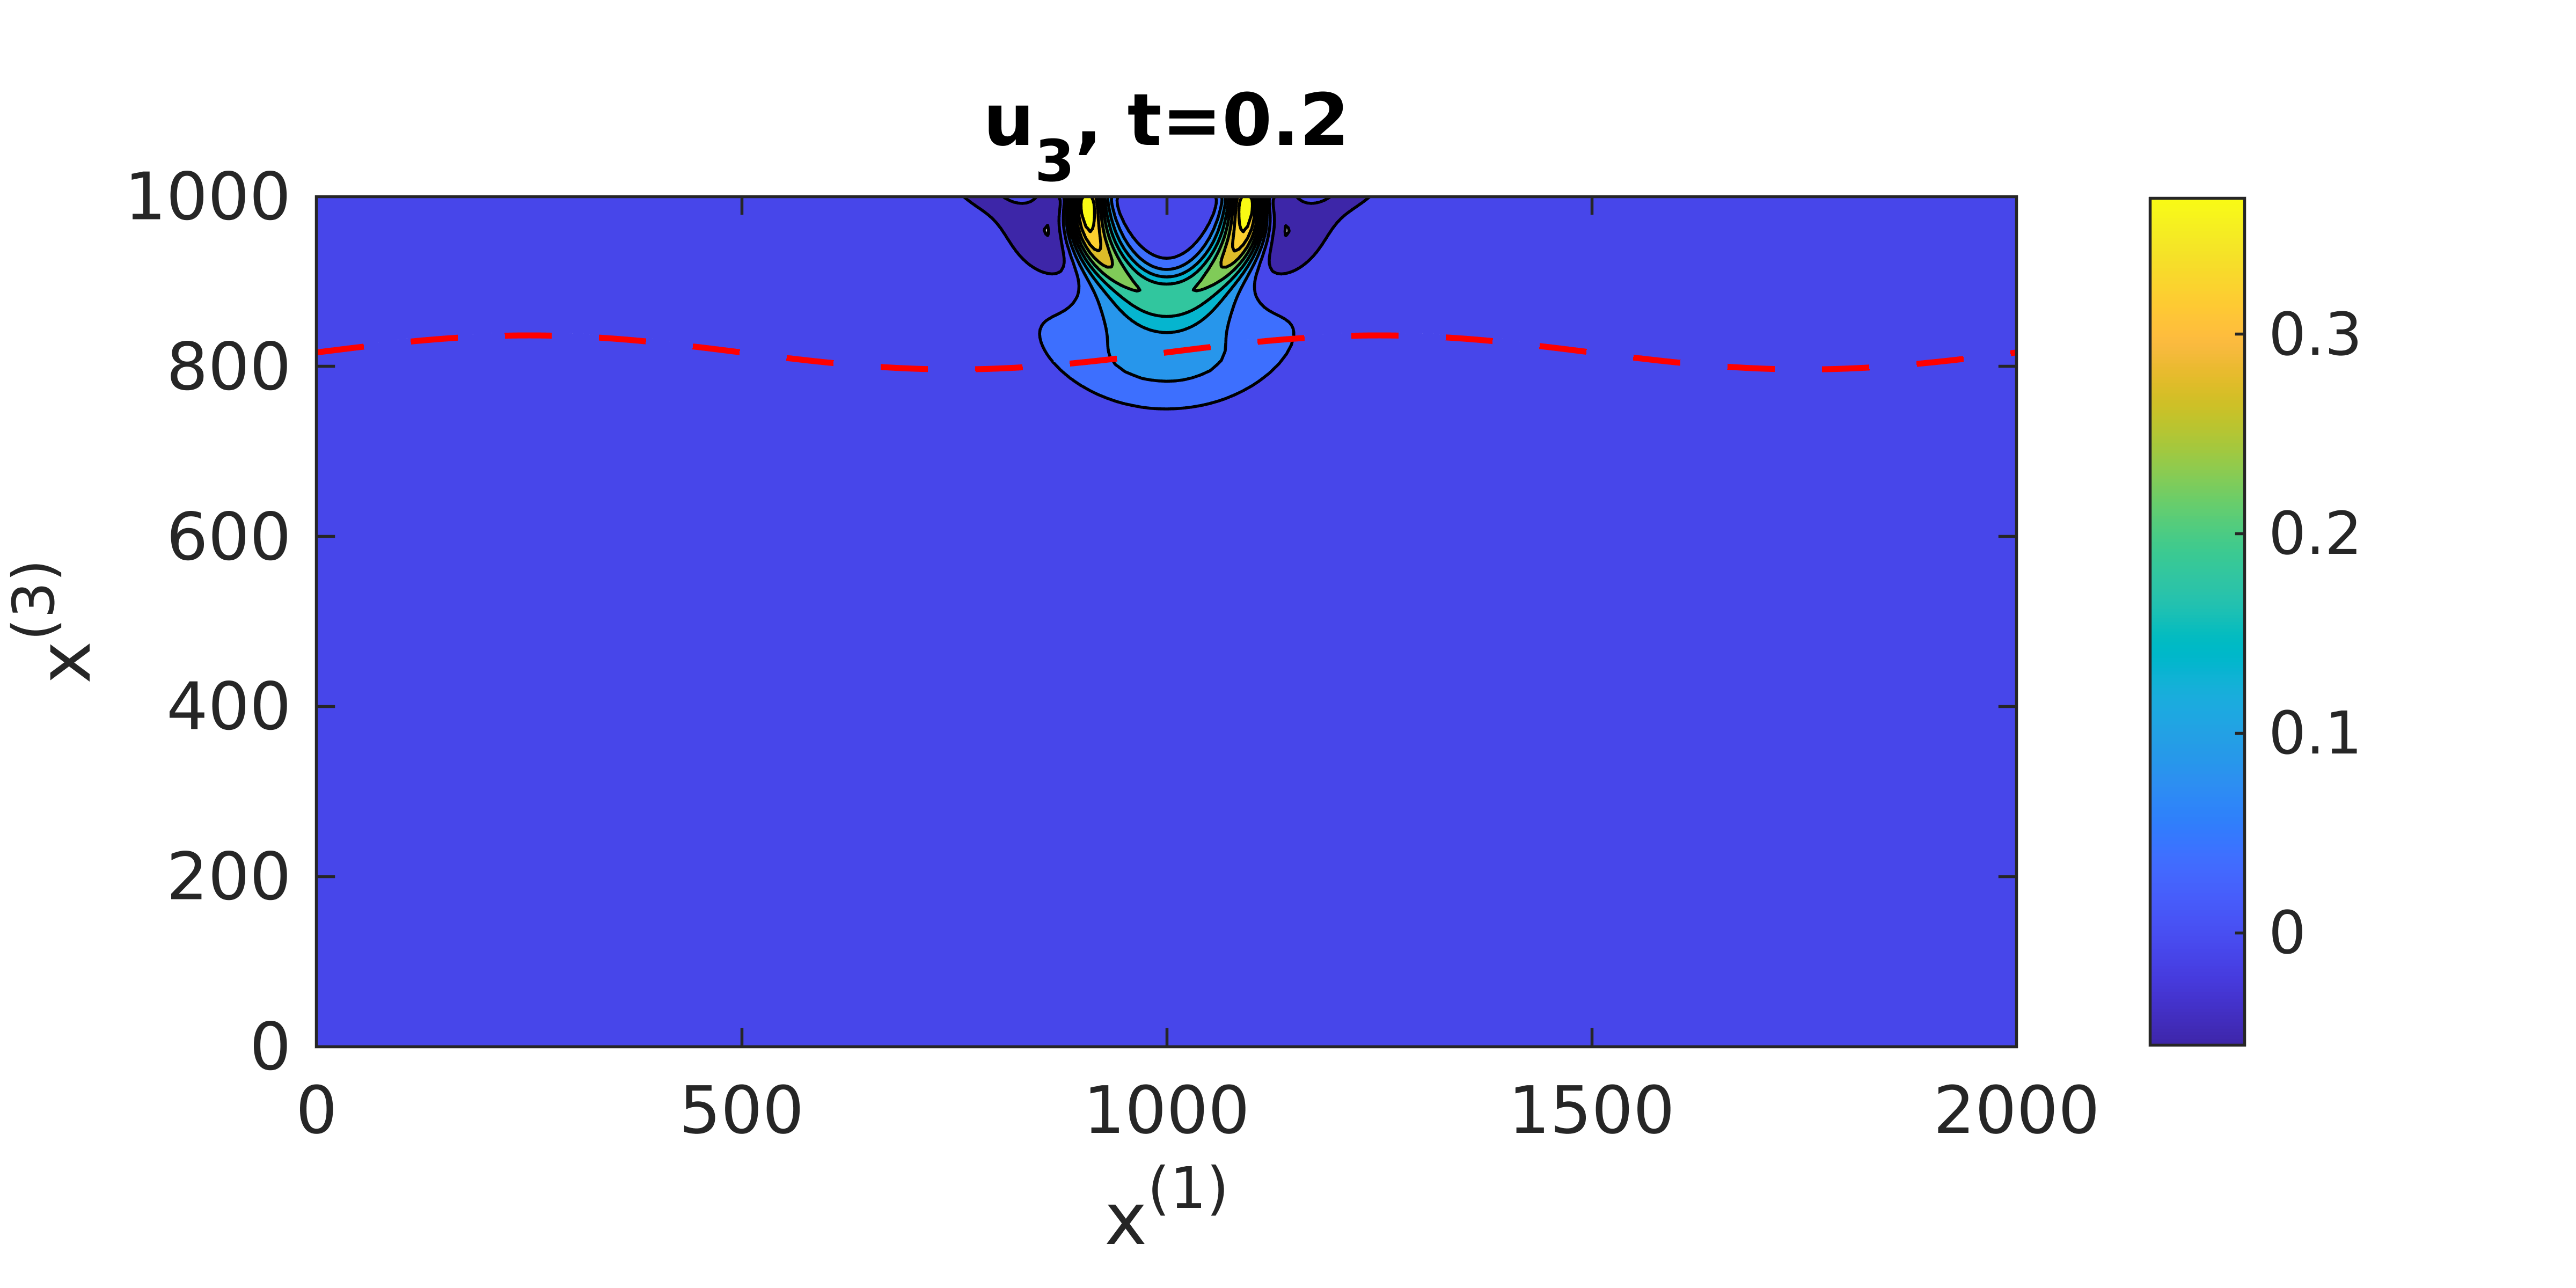
\includegraphics[width=0.49\textwidth,trim={0.05cm 0.1cm 0.55cm 0.45cm}, clip]{u3_t02_curvi_finer.png}
	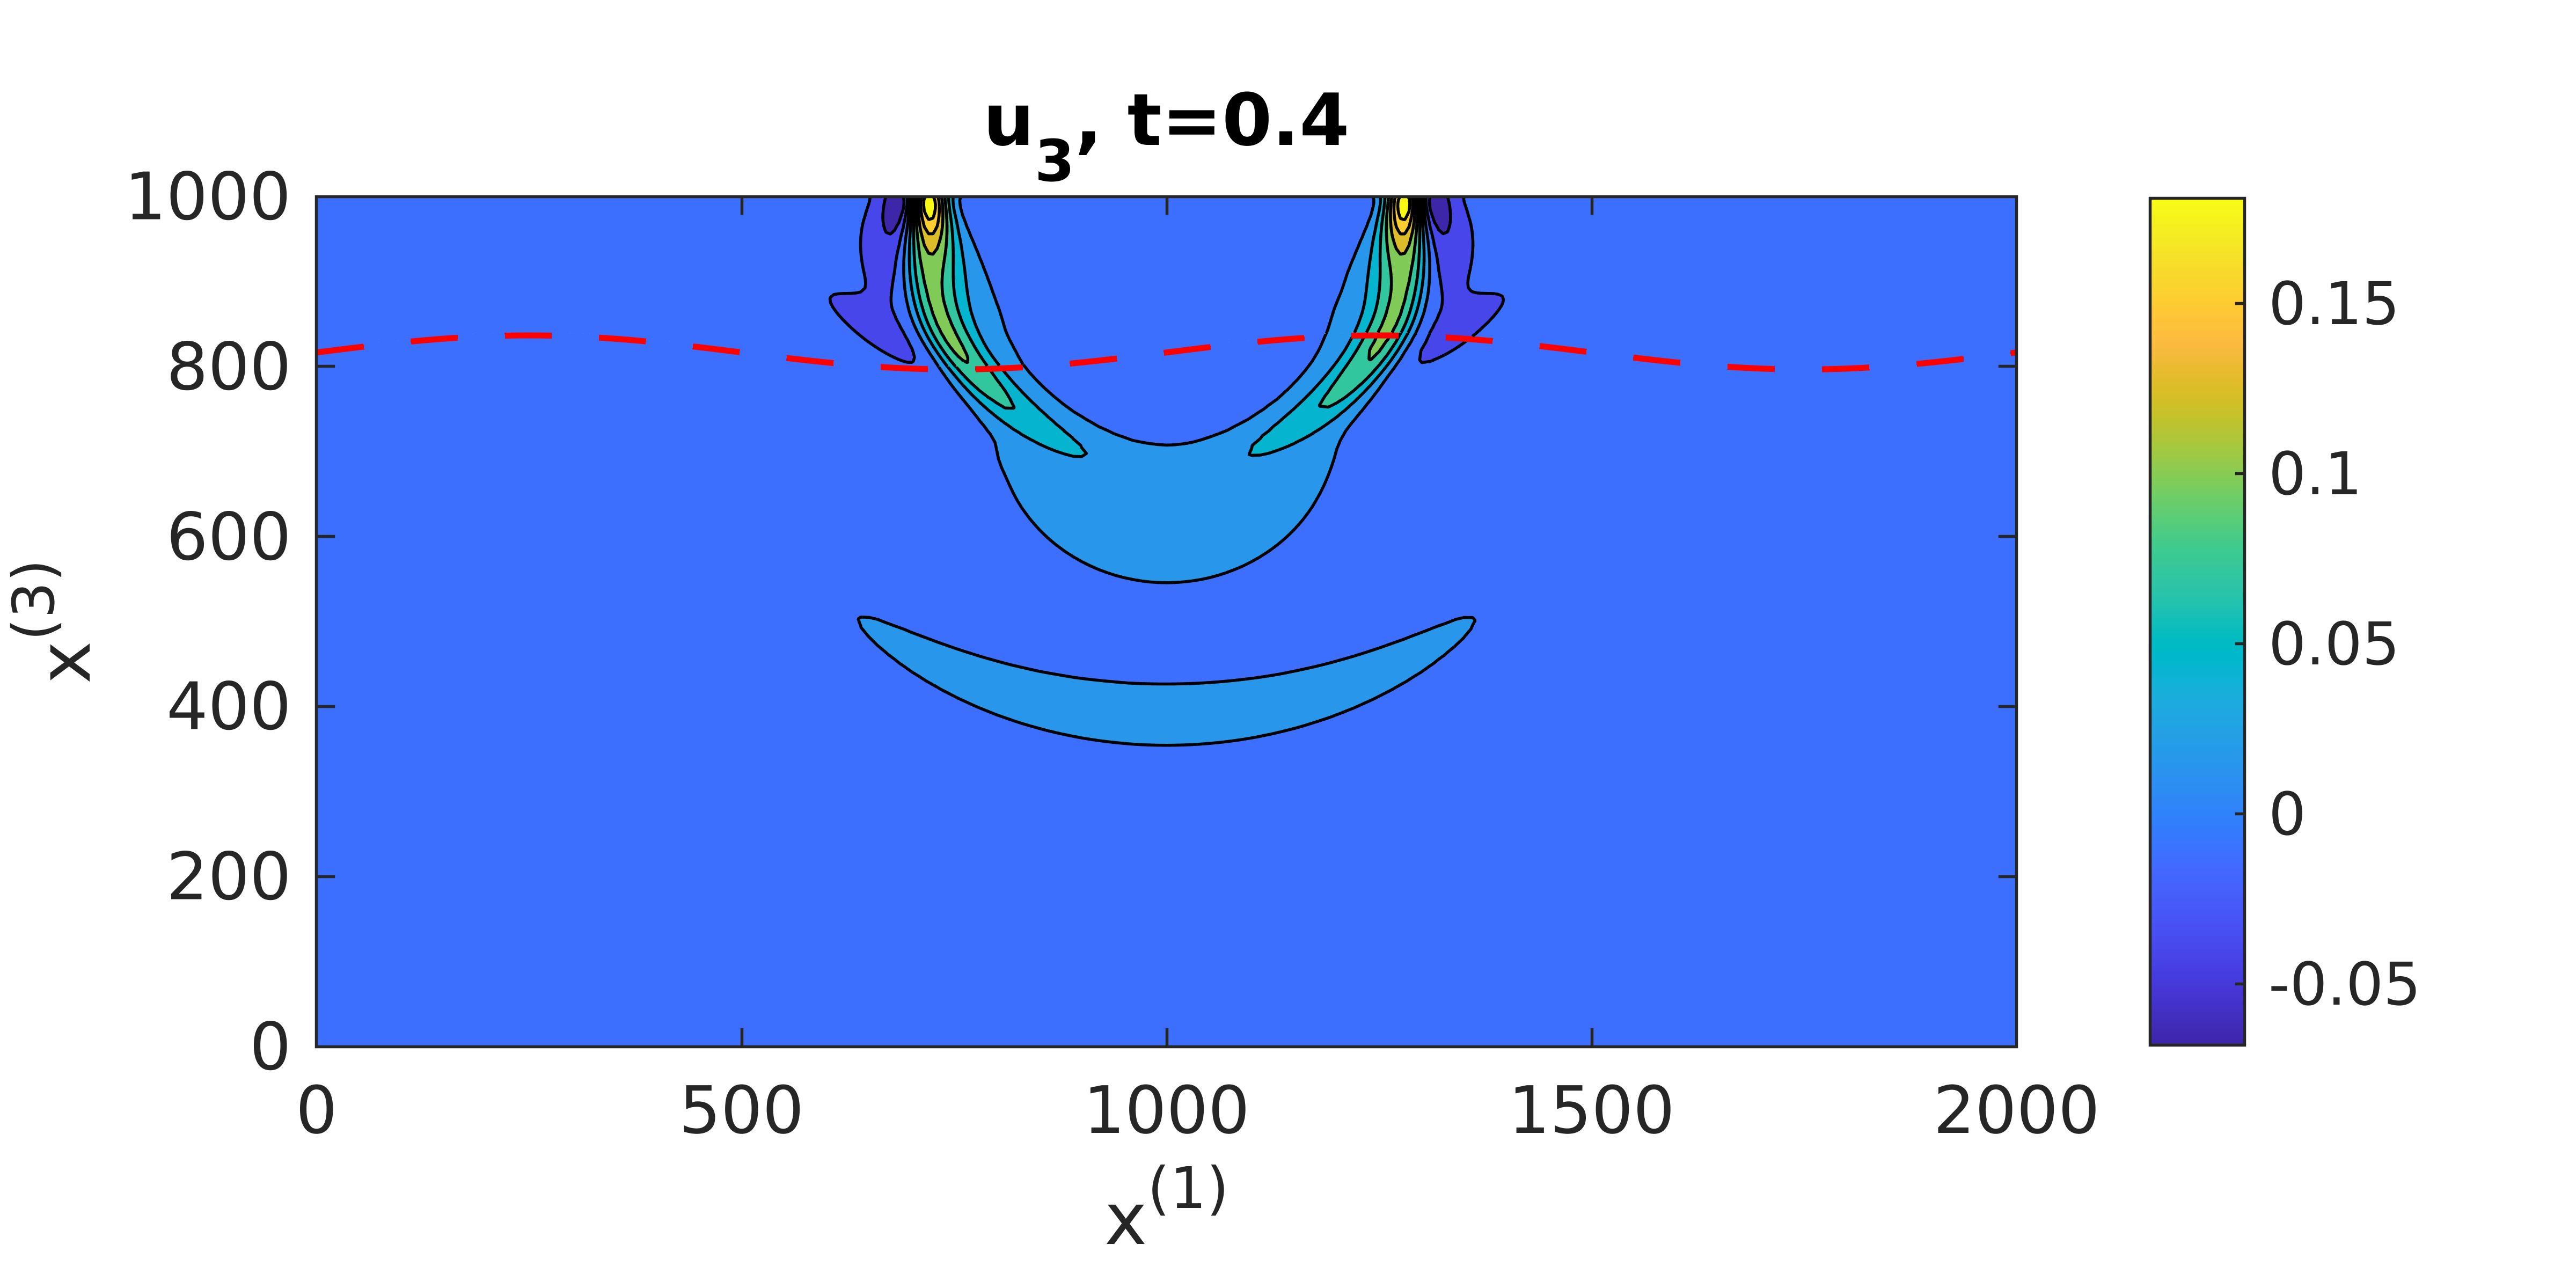
\includegraphics[width=0.49\textwidth,trim={0.05cm 0.1cm 0.55cm 0.45cm}, clip]{u3_t04_curvi_finer.png}
	\caption{The graphs for $u_3$. In the top, middle and bottom panel, we show numerical solutions at $t=0.2$ and $t=0.4$ computed with Mesh 1, Mesh 2 and Mesh 3, respectively. The curved interfaces are marked with the red dash lines.}
\label{u3}
\end{figure}
In Figure \ref{u1}, we plot the component $u_1$ at $t=0.2$ and $t=0.4$.  Some artifacts are observed in the solution computed with the second mesh, which is due to the small number of grid points per wavelength in $\Omega^c$. The results become better when the finer curvilinear mesh is used. From Figure \ref{u3}, we observe that there is no obvious reflection at the mesh refinement interface for the component $u_3$, and we have a better results when a finer curvilinear mesh is used. The component $u_2$ is zero up to round-off error for both the Cartesian mesh and curvilinear meshes and is not presented here.